\documentclass[11pt]{charter}
\usepackage{pdflscape}
% El títulos de la memoria, se usa en la carátula y se puede usar el cualquier lugar del documento con el comando \ttitle
\titulo{Sistema de monitoreo de temperaturas en tiempo real para refrigeradores críticos de salud} 

% Nombre del posgrado, se usa en la carátula y se puede usar el cualquier lugar del documento con el comando \degreename
%\posgrado{Carrera de Especialización en Sistemas Embebidos} 
\posgrado{Carrera de Especialización en Internet de las Cosas} 
%\posgrado{Carrera de Especialización en Intelegencia Artificial}
%\posgrado{Maestría en Sistemas Embebidos} 
%\posgrado{Maestría en Internet de las cosas}

% Tu nombre, se puede usar el cualquier lugar del documento con el comando \authorname
\autor{Marcelo Castello} 

% El nombre del director y co-director, se puede usar el cualquier lugar del documento con el comando \supname y \cosupname y \pertesupname y \pertecosupname
\director{Juan José Salerno}
\pertenenciaDirector{UTN - FRRO} 
% FIXME:NO IMPLEMENTADO EL CODIRECTOR ni su pertenencia
\codirector{} % si queda vacio no se deberíá incluir 
\pertenenciaCoDirector{}

% Nombre del cliente, quien va a aprobar los resultados del proyecto, se puede usar con el comando \clientename y \empclientename
\cliente{Edgardo Marino}
\empresaCliente{Municipalidad de Rosario}

% Nombre y pertenencia de los jurados, se pueden usar el cualquier lugar del documento con el comando \jurunoname, \jurdosname y \jurtresname y \perteunoname, \pertedosname y \pertetresname.
\juradoUno{Nombre y Apellido (1)}
\pertenenciaJurUno{pertenencia (1)} 
\juradoDos{Nombre y Apellido (2)}
\pertenenciaJurDos{pertenencia (2)}
\juradoTres{Nombre y Apellido (3)}
\pertenenciaJurTres{pertenencia (3)}
 
\fechaINICIO{25 de agosto de 2020}		%Fecha de inicio de la cursada de GdP \fechaInicioName
\fechaFINALPlanificacion{6 de octubre de 2020} 	%Fecha de final de cursada de GdP
\fechaFINALTrabajo{13 de abril de 2021}		%Fecha de defensa pública del trabajo final


\begin{document}

\maketitle
\thispagestyle{empty}
\pagebreak


\thispagestyle{empty}
{\setlength{\parskip}{0pt}
\tableofcontents{}
}
\pagebreak


\section{Registros de cambios}
\label{sec:registro}


\begin{table}[ht]
\label{tab:registro}
\centering
\begin{tabularx}{\linewidth}{@{}|c|X|c|@{}}
\hline
\rowcolor[HTML]{C0C0C0} 
Revisión & \multicolumn{1}{c|}{\cellcolor[HTML]{C0C0C0}Detalles de los cambios realizados} & Fecha      \\ \hline
1.0      & Creación del documento \newline Versión inicial: propósito, alcance, supuestos, requerimientos, entregables y desglose del trabajo.
                                         & 26/08/2020 \\ \hline
1.2      & Primera entrega                                                                 & 04/09/2020 \\ \hline
1.3      & Primera corrección &15/06/2020\\\hline
%		   Con texto partido \newline
%		   En varias líneas \newline
%		   A propósito                                                     & dd/mm/aaaa \\ \hline
\end{tabularx}
\end{table}

\pagebreak



\section{Acta de constitución del proyecto}
\label{sec:acta}

\begin{flushright}
Buenos Aires, \fechaInicioName
\end{flushright}

\vspace{2cm}

Por medio de la presente se acuerda con el Ing. \authorname\hspace{1px} que su Trabajo Final de la \degreename\hspace{1px} se titulará ``\ttitle'', consistirá esencialmente en el prototipo preliminar de un sistema para la medición, visualización y emisión de alertas de temperatura para heladeras y freezers en bancos de sangre y vacunatorios de efectores de salud de la Municipalidad de Rosario, y tendrá un presupuesto preliminar estimado de 663 hs de trabajo y {\$731120}, con fecha de inicio \fechaInicioName\hspace{1px} y fecha de presentación pública \fechaFinalName.

Se adjunta a esta acta la planificación inicial.

\vfill

% Esta parte se construye sola con la información que hayan cargado en el preámbulo del documento y no debe modificarla
\begin{table}[ht]
\centering
\begin{tabular}{ccc}
\begin{tabular}[c]{@{}c@{}}Ariel Lutenberg \\ Director posgrado FIUBA\end{tabular} & \hspace{2cm} & \begin{tabular}[c]{@{}c@{}}\clientename \\ \empclientename \end{tabular} \vspace{2.5cm} \\ 
\multicolumn{3}{c}{\begin{tabular}[c]{@{}c@{}} \supname \\ Director del Trabajo Final\end{tabular}} \vspace{2.5cm} \\
%\begin{tabular}[c]{@{}c@{}}\jurunoname \\ Jurado del Trabajo Final\end{tabular}     &  & \begin{tabular}[c]{@{}c@{}}\jurdosname\\ Jurado del Trabajo Final\end{tabular}  \vspace{2.5cm}  \\
%\multicolumn{3}{c}{\begin{tabular}[c]{@{}c@{}} \jurtresname\\ Jurado del Trabajo Final\end{tabular}} \vspace{.5cm}                                                                     
\end{tabular}
\end{table}




\section{Descripción técnica-conceptual del proyecto a realizar}
\label{sec:descripcion}

\begin{consigna}{black}
%El objetivo es que el lector en una o dos páginas entienda de qué se trata el proyecto y cuáles son sus desafíos, su motivación y su importancia.
%Se debe destacar claramente cuál es el valor que agrega el proyecto a realizar. ``El presente proyecto se destaca especialmente por incorporar tal cosa... Esto lo diferencia de otros sistemas similares en que ...''
El presente proyecto, está dirigido a solucionar un problema existente en la Municipalidad de Rosario, donde en el área Salud Pública, funcionan  hospitales, centros de salud, droguerías y bancos de sangre. Todos estos efectores necesitan para almacenar los insumos médicos sistemas de refrigeración que provean alta confiabilidad en su prestación.

El buen funcionamiento de estos sistemas es afectado a menudo por cortes de energía, mermas en el rendimiento del equipo compresor, o pérdidas en el sello ya sea por desgaste de burletes o puertas mal cerradas.
En el área de salud esto resulta crítico. Productos medicinales como hemoproductos o vacunas, pueden perder la eficacia médica. Esto no sólo se traduce en pérdidas económicas, sino también implica que los tratamientos sobre las personas pueden no ser efectivos o que no puedan ser accedidos por la pérdida del material, con el consecuente impacto social y mediático que esto representa para el municipio.

%Los cortes de energía que se producen a menudo en la red eléctrica afectan de manera directa el buen funcionamiento de los sistemas de refrigeración, sean de productos medicinales como de hemoproductos, pudiendo en algunos casos perder la cadena de frío con la consiguiente pérdida del material almacenado. Esto no sólo se traduce en pérdidas económicas, sino también implica que personas no puedan acceder a los tratamientos o vacunas con el consecuente impacto social y mediático que esto representa en una empresa pública. 
Además, la Administración Nacional de Medicamentos Alimentos y Tecnología Médica (ANMAT), a través de la disposición: "Reglamento Técnico Mercosur sobre Buenas Prácticas de Distribución de Productos Farmacéuticos", Resolución Mercosur GMC Nº 49/2002, define un conjunto de prácticas para el transporte y almacenamiento de productos farmacéuticos donde exige trazabilidad, equipamiento para el control y registro continuo de temperaturas con el fin de asegurar las condiciones ambientales de almacenamiento de tales productos. 

La medición a distancia continua y en tiempo real de estas temperaturas sumado a un sistema de alerta, aseguran las condiciones legales, minimizan los riesgos y garantizan la disponibilidad de hemoproductos y vacunas seguros en el momento y el lugar en que se precise. 

Este tabajo se enmarca en dos premisas fundamentales:
\begin{itemize}
\item La misión de la Secretaría de Salud Pública es preservar la salud de la población y proponer un trabajo integrador para la construcción de opciones y entornos saludables.
\item El contexto sanitario mundial de hoy exige que en un futuro cercano se puedan distribuir adecuadamente y de manera segura especialidades medicinales tales como las vacunas.
\end{itemize}
Los equipos y software de que se dispone en plaza en su mayoría son de origen extranjero, y su utilización -además de onerosa- implica una dependencia con los fabricantes, en términos económicos pero también de criterios (en general se comercializan por módulos, no proveyendo soluciones integrales). En otras palabras, para trabajar con estos recursos se deben seguir criterios técnico-económicos diseñados para otras latitudes y otras condiciones. Se deben realizar adaptaciones y aproximaciones que implican tareas adicionales y que no siempre son del todo efectivas. El personal destinado a estas tareas debe entrenarse utilizando tiempo y esfuerzo, y este entrenamiento debe reforzarse cada vez que el propietario del sistema decide algún cambio o actualización. Por consiguiente, es menester redirigir este esfuerzo a tareas más provechosas.
Se requiere para ello el desarrollo de tecnología propia destinada a este fin, que pueda ser adaptada a las necesidades de los investigadores locales, para evitar la dependencia tecnológica en equipos y en software, y reducir en todo lo posible las erogaciones durante la investigación por este ítem.

Desde el punto de vista tecnológico, el presente proyecto se destaca especialmente por incorporar una solución integral sin gastos de abono y con la característica distintiva que los datos están guardados en los servidores del cliente. Esto lo diferencia de otros sistemas similares en que los datos quedan en poder del fabricante, quien eventualmente, ofrece un portal para poder hacer una visualización. Además, al no ofrecer una solución integral, cada módulo extra incorporado representa un gasto o abono adicional. 

La solución propuesta se compone de las siguientes partes:
\begin{itemize}
\item Medición de la temperatura
\item Transporte de los datos
\item Lógica de procesamiento y persistencia de datos
\item Visualización y alarmas
\end{itemize}
%Puede ser útil incluir en esta sección la respuesta a alguna de estas preguntas:


%La descripción técnica-conceptual \textbf{debe incluir al menos un diagrama en bloques del sistema }y una frase como la siguiente: ``En la Figura \ref{fig:diagBloques} se presenta el diagrama en bloques del sistema. Se observa que...''. Luego recién más abajo de haber puesto esta frase se pone la figura. La regla es que las figuras nunca pueden ir antes de ser mencionadas en el texto, porque sino el lector no entiende por qué de pronto aparece una figura.
En la figura 1 se observa un diagrama en bloques general del sistema, donde se aprecia que los sensores estarán ubicados en distintos efectores del sistema de salud municipal en las áreas de hemoterapia y vacunación. Además se puede ver el sistema de almacenamiento y visualización implementado con un tablero de control  (dashboard) en un servidor centralizado ubicado en el datacenter de la Secretaría de Salud Pública. Por simplicidad, se han dibujado sólo tres efectores. 

Es necesario precisar lo antes mencionado. El sistema de salud pública municipal de la ciudad de Rosario consta de 6 hospitales, un centro de especialidades médicas, un centro regional de sangre, una droguería central y 50 centros de atención primaria de la salud.
\vspace{25px}

\begin{figure}[htpb]
\centering 
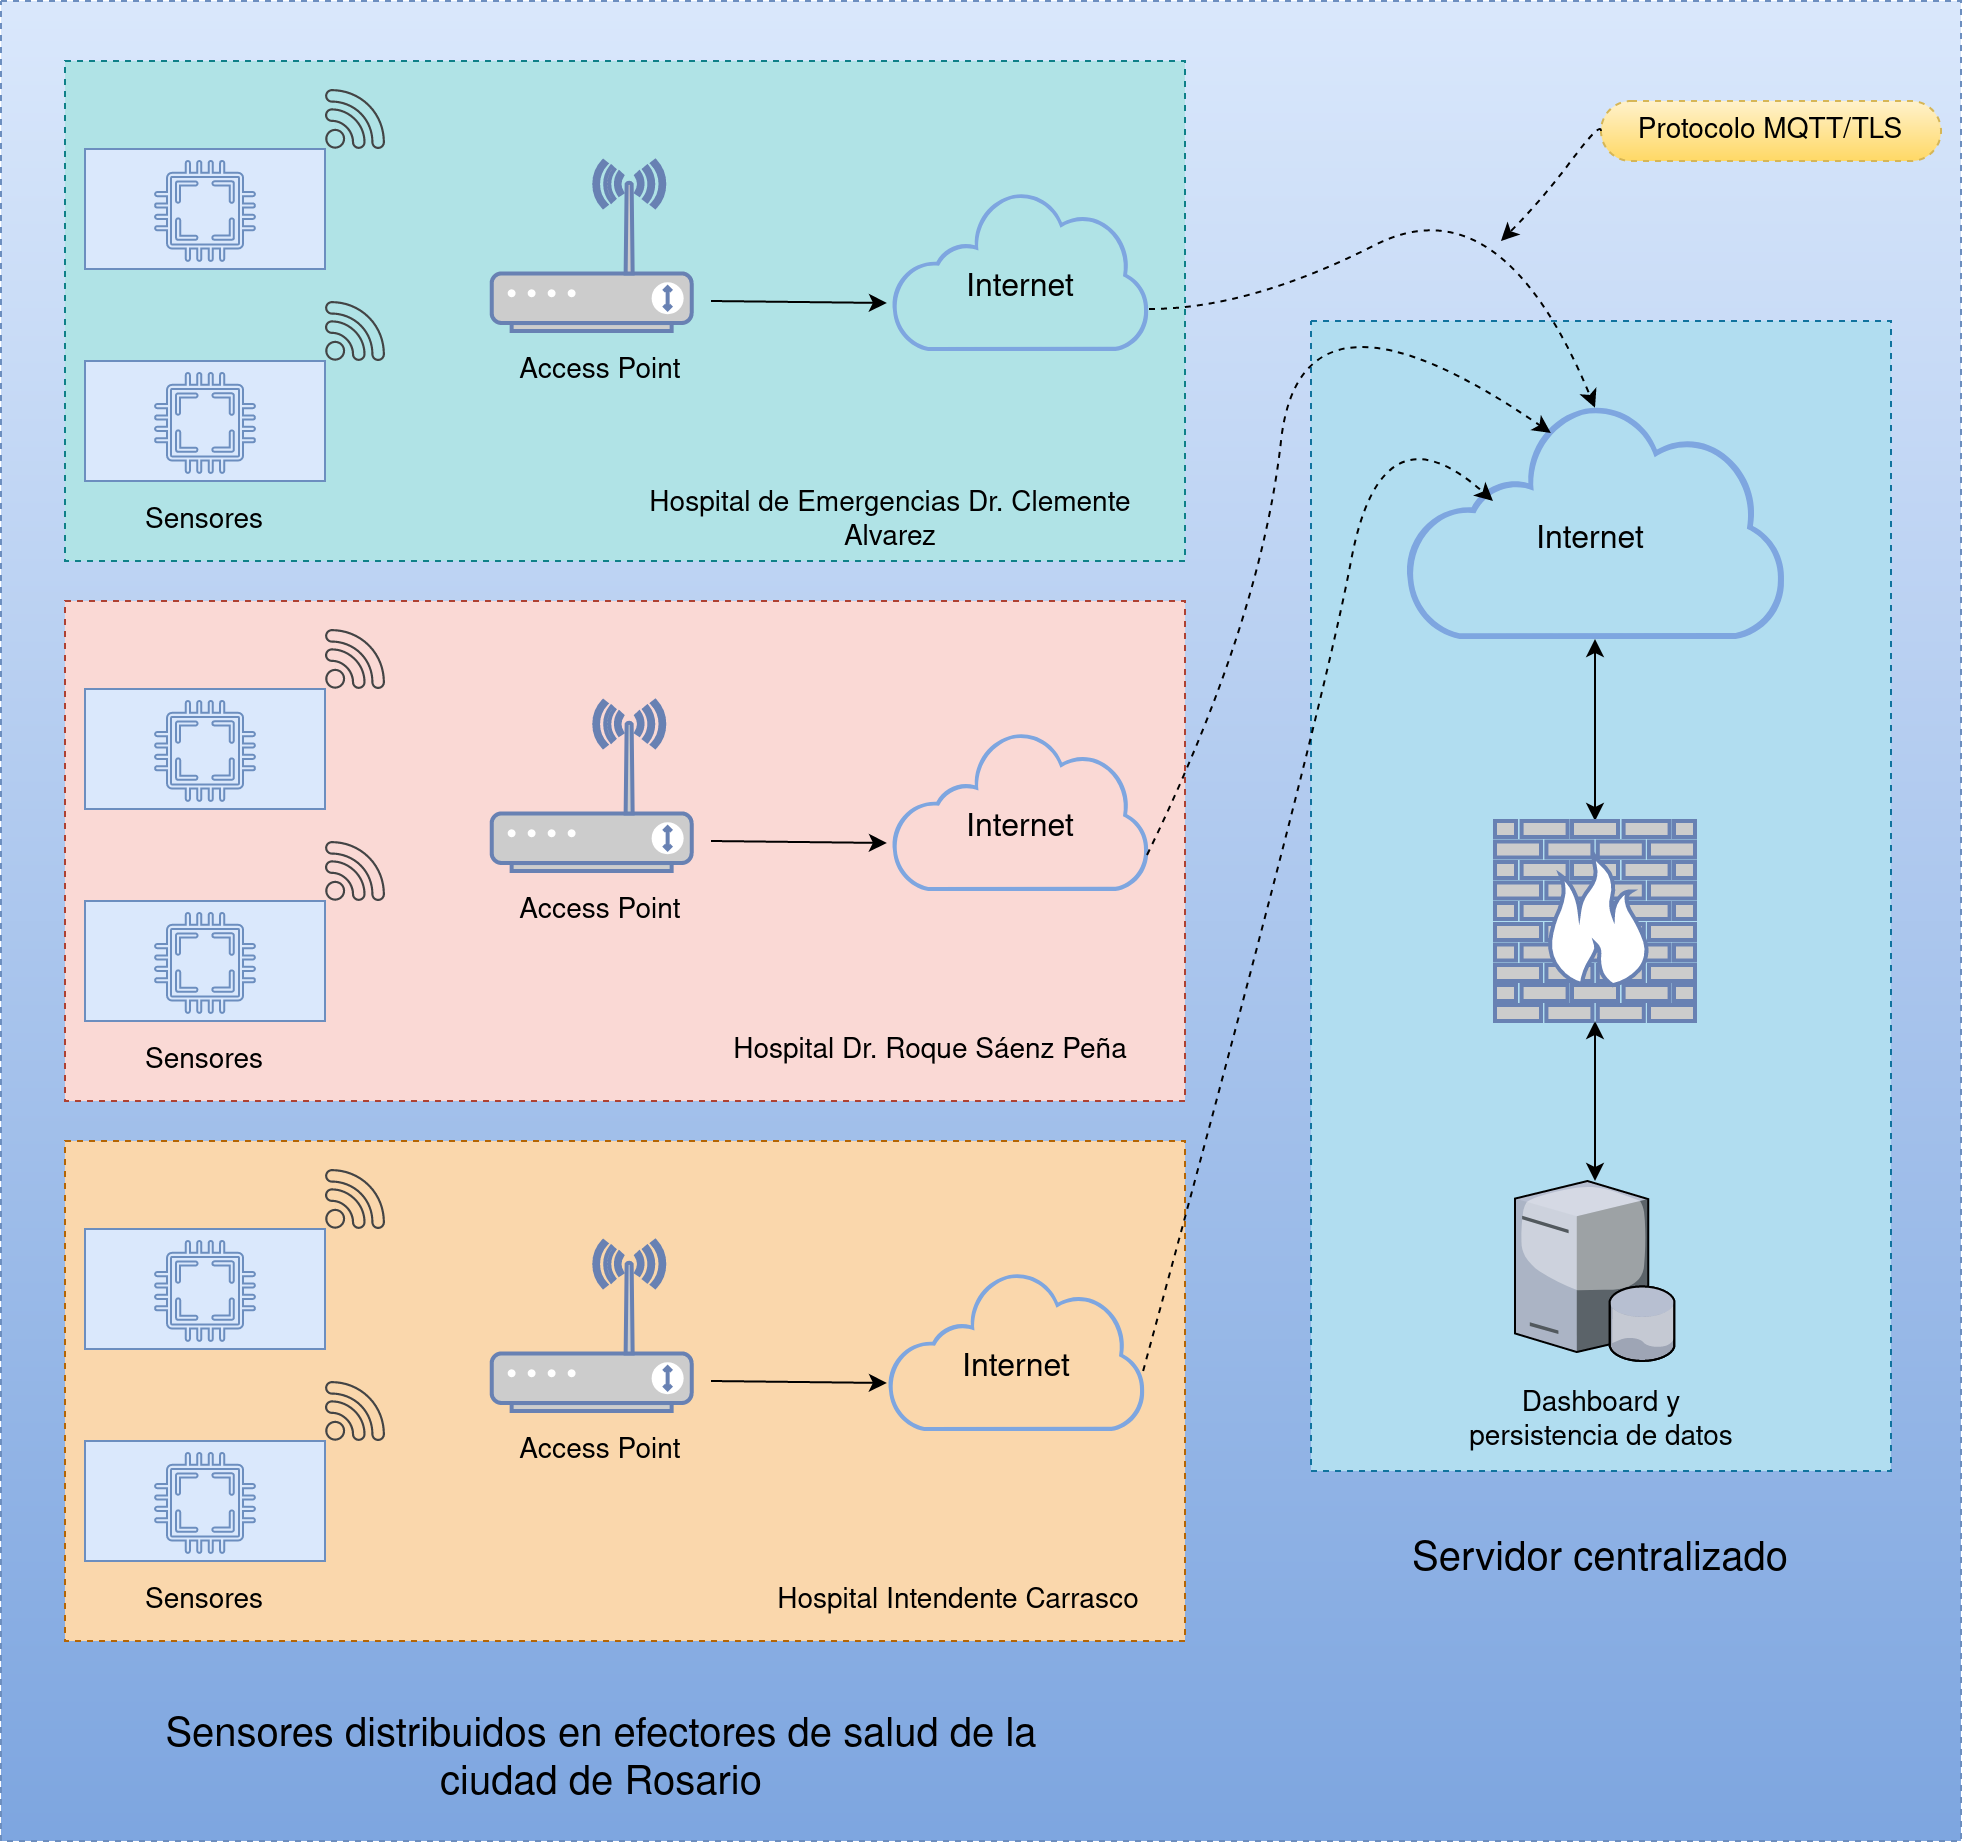
\includegraphics[width=.9\textwidth]{./Figuras/bloquesgral.png}
\caption{Diagrama en bloques del sistema}
\label{fig:diagBloques}
\end{figure}

\vspace{25px}

%El tamaño de la tipografía en la figura debe ser adecuado para que NO pase lo que ocurre acá, donde el lector debe esforzarse para poder leer el texto. Los colores usados en el diagrama deben ser adecuados, tal que ayuden a comprender mejor el diagrama.
\end{consigna}


\section{Identificación y análisis de los interesados}
\label{sec:interesados}

\begin{consigna}{black} 
%Nota: (borrar esto y todas las consignas en color rojo antes de entregar este documento).
 
%Es inusual que una misma persona esté en más de un rol, incluso en proyectos chicos.
 
%Si se considera que una persona cumple dos o más roles, entonces sólo dejarla en el rol más importante. Por ejemplo:

%\begin{itemize}
%\item Si una persona es Cliente pero también colabora u orienta, dejarla solo como Cliente.
%\item Si una persona es el Responsable, no debe ser colocado también como Miembro del equipo.
%\end{itemize}

%Pero en cambio sí es usual que el Cliente y el Auspiciante sean el mismo, por ejemplo.

\begin{table}[ht]
%\caption{Identificación de los interesados}
%\label{tab:interesados}
\begin{tabularx}{\linewidth}{@{}|l|X|X|l|@{}}
\hline
\rowcolor[HTML]{C0C0C0} 
Rol           & Nombre y Apellido & Organización 	& Puesto 	\\ \hline
%Auspiciante   &                   &              	&    -    	\\ \hline
Cliente       & \clientename      &\empclientename	&      Director de Bioingeniería\\ \hline
Impulsor y colaborador      & Roberto Collelo  & \empclientename	&Sub Director de Bioingeniería\\ \hline
Responsable   & \authorname       & FIUBA        	& Alumno 	\\ \hline
Colaboradores & 
                Silvana Pereyra &Dirección Centros de Salud	 &Jefa Droguería Central\\ \hline
Orientador    & \supname	      & \pertesupname 	& Director	Trabajo final \\ \hline
%Equipo        & miembro1 \newline 
%				miembro2          &       -       	&      -  	\\ \hline
%Opositores    &    -               &      -        	&     -   	\\ \hline
%Usuario final &      -             &      -        	&      -  	\\ \hline
\end{tabularx}
\end{table}


%Sería deseable listar a continuación de la tabla las principales características de cada interesado.
 
%Por ejemplo:
\begin{itemize}
%\item Auspiciante: es riguroso y exigente con la rendición de gastos. Tener mucho cuidado con esto.
%\item Equipo: Juan Perez, suele pedir licencia porque tiene un familiar con una enfermedad. Planificar considerando esto.
\item Colaboradores

Roberto Collelo: resulta de valiosa ayuda en el desarrollo del firmware de los sensores, además de promover el proyecto en las estructuras de mando de la Secretaría de Salud Pública.

Silvana Pereyra: su intervención será desde el lado usuarios, ya que se muestra como una facilitadora para la implementación del sistema.
\end{itemize}

\end{consigna}



\section{1. Propósito del proyecto}
\label{sec:proposito}

\begin{consigna}{black}
El propósito de este proyecto es poner en marcha un sistema de registro y visualización de temperaturas para refrigeradores críticos del área salud, con el objetivo de minimizar los riesgos de pérdida de material, mantener la calidad y eficacia médica de los productos y asegurar las condiciones legales exigidas por la autoridad.
\end{consigna}

\section{2. Alcance del proyecto}
\label{sec:alcance}

\begin{consigna}{black}
El presente proyecto incluye el desarrollo de sus partes fundamentales para que sea capaz de tener una vigilancia de temperatura de al menos 4 heladeras pertenecientes a distintos efectores de salud de la ciudad de Rosario. 
Para ello se desarrollarán y producirán las placas de circuito impreso para los sensores de temperatura, se integrarán en una caja plástica para poder ser colocados en el equipamiento a monitorear.

Se instalará y configurará en un servidor con sistema operativo GNU/Linux con distribución Debian, la dashboard Thingsboard versión Community Edition que es la versión libre de licenciamientos pero que contiene todas las funcionalidades necesarias para este proyecto.

Se configurarán reglas en la dashboard para comparar las temperaturas de los dispositivos con sus rangos para así originar las alarmas y enviar las notificaciones.

Se instalará una base de datos en el servidor central donde se almacenarán las temperaturas, y las configuraciones del sistema.

Se configurarán en la dashboard paneles para que proporcionen información de temperatura y estado para cada dispositivo conectado al sistema.

Las notificaciones de alarmas se harán por medio de la red Telegram, configurando un canal para cada efector/área.


El presente proyecto no incluye la provisión de la infraestructura de transporte de datos, esto es, los equipos para puntos de acceso a Internet y las conexiones a Internet para cada área donde estarán emplazados los sensores. Tampoco incluirá certificaciones emitidas por las autoridades competentes.
Los sensores desarrollados no son aptos para su instalación en equipos ultrafreezer (-70º).
Los sensores no almacenarán los valores de temperaturas en memorias externas tipo SD ni en la memoria interna del microcontrolador.
Los sensores no usarán baterías para su funcionamiento.

\end{consigna}


\section{3. Supuestos del proyecto}
\label{sec:supuestos}

\begin{consigna}{black}
Para el desarrollo del presente proyecto se supone que:

\begin{itemize}
\item Las áreas donde se colocarán los sensores deberán disponer de una conexión a Internet.
\item Para la puesta en producción, se utilizará la infraestructura de servidores de la red informática metropolitana de la ciudad de Rosario
\item Los recursos humanos y el tiempo necesario para el desarrollo serán proporcionados por la Municipalidad de Rosario.
\item El gasto producido por la compra de los elementos necesarios será proporcionado por la Municipalidad de Rosario.
\end{itemize}

\end{consigna}

\section{4. Requerimientos}
\label{sec:requerimientos}

\begin{consigna}{black}
Se presentan a continuación los requerimientos del proyecto, los mismos están presentados en funcionales y no funcionales, donde los ítems de cada requerimiento están priorizados por orden de aparición.

Estos requerimientos se obtuvieron por:
\begin{itemize}
\item Relevamiento de las espectativas de los usuarios.
\item Relevamiento de las condiciones impuestas por el cliente.
\item Estudio de los elementos electrónicos disponibles en el mercado local y extranjero.
\item Ordenanza de contabilidad de la Municipalidad de Rosario.
\end{itemize}

\begin{enumerate}
\item Requerimientos de hardware de los nodos
	\begin{enumerate}
	\item Cada nodo estará compuesto por un microcontrolador un elemento sensor de temperatura y la electrónica asociada para su funcionamiento.
	\item El microcontrolador utilizado deberá estar en fase de producción activa.
	\item El microcontrolador deberá contener capa física WiFi.	
	\item El elemento sensor deberá tener un rango de medición entre -50 y 100 ºC
	\item El nodo deberá incluir en su circuito un filtro activo de 2º orden para la filtrar las componentes de alta frecuencia de la entrada de temperatura.
	\item El nodo deberá incorporar indicadores luminosos de conexión con la red WiFi, conexión con el servidor central e indicador de fuera de rango de temperatura.	
	\end{enumerate}
	
\item Requerimientos del software de los nodos
	\begin{enumerate}
	\item Deberá contener un conjunto de parámetros que identifiquen de forma unívoca el sensor dentro del sistema.	
	\item Los parámetros se deberán almacenar en memoria no volátil.
	\item Deberá gestionar el procesamiento de los valores de temperatura: muestreo cada segundo y promediado cada 600 segundos.	
	\item Deberá incluir parámetros de calibración como offset y ganancia para su futuro contraste con un instrumento patrón.
	\item El nodo deberá incorporar una página web para configuración de parámetros específicos/calibración del sensor.
	\item Deberá incorporar un sistema de actualización remota del firmware.
    \item Deberá ser capaz de conectar distintos modelos de sensores de temperatura.
	\end{enumerate}	
	
\item Requerimientos de seguridad informática
	\begin{enumerate}
	\item La transmisión de los datos se deberá realizar con encriptación, utilizando para ello protocolos de seguridad.
	\item El acceso al sistema de visualización deberá ser con usuario y contraseña.
	\item El acceso a la página web del sensor deberá ser con usuario y contraseña.
	\end{enumerate}	

\item Requerimientos del cliente
	\begin{enumerate}
	\item El sistema de visualización debe incluir roles para distintos usuarios.
		\begin{enumerate}
		\item Rol Administrador: podrá dar alta a usuarios y cambiar sus roles.
	     \item Rol Jefe: podrá cambiar parámetros, visualizar series de tiempo y recibir alertas.
	     \item Rol Operador: sólo podrá visualizar series de tiempo y recibir alertas.
	     \end{enumerate}
	\item El sistema deberá prever la incorporación de otras variables a monitorear, que serán materia de desarrollos futuros de sensores.
	\item El sistema de visualización deberá mostrar claramente la estructura jerárquica geográfica de la empresa.	
	\item El sistema deberá ser escalable para implementar nuevas áreas a monitorear.
		\end{enumerate}
		
\item Requerimientos del sistema de visualización
    \begin{enumerate}
	\item Deberá mostrar la temperatura.
	\item Deberá mostrar el estado del dispositivo. (online/fuera de rango)
	\item Deberá mostrar la fecha y hora de la última telemetría enviada al servidor.
	\item Deberá mostrar la configuración de los parámetros de alertas (rangos de temperatura).
	\item Deberá mostrar una vista rápida de los sensores fuera de rango mediante plano en pantalla del área.
	\item Deberá mostrar una tabla con el histórico de alarmas por cada sensor.
    \item Deberá mostrar mediante gráficas la evolución de las temperaturas en el dominio del tiempo con entorno configurable.
    \item Deberá mostrar el lugar de emplazamiento del dispositivo.
	\end{enumerate}	
    

\item Requerimientos de las alarmas
	\begin{enumerate}
	\item Deberá enviar las alarmas discriminadas por efector/área.
	\item Deberá enviar notificaciones ante desplazamientos de la temperatura por encima del rango.
	\item Deberá enviar notificaciones ante desplazamientos de la temperatura por debajo del rango.
	\item Deberá enviar notificaciones ante desconexiones del dispositivo sensor.
	\item Deberá enviar notificaciones ante recupero de la conexión del dispositivo sensor.
	 \end{enumerate}	 

\item Requerimientos de compras
	\begin{enumerate}
	\item Se deberá utilizar la gestión de compras directas para elementos con presupuesto menor a {\$10.000}.
	\item Se deberán realizar las gestiones correspondiente para realizar compras en el exterior.
	\end{enumerate}
	
%\item Requierimientos de normativas
%	\begin{enumerate}
%	\item 
%	\item 
%	\end{enumerate}
		
\end{enumerate}


\end{consigna}

\section{Historias de usuarios (\textit{Product backlog})}
\label{sec:backlog}

\begin{consigna}{black}
%Descripción: En esta sección se deben incluir las historias de usuarios y su ponderación (\textit{history points}). Recordar que las historias de usuarios son descripciones cortas y simples de una característica contada desde la perspectiva de la persona que desea la nueva capacidad, generalmente un usuario o cliente del sistema. La ponderación es un número entero que representa el tamaño de la historia comparada con otras historias de similar tipo.
Se muestran a continuación, las historias de usuarios recopiladas. Al principio se presentan dos épicas y sus correspondientes desgloses emanadas de las máximas autoridades de la empresa.

La ponderación de estas historias se realizó teniendo en cuenta la complejidad y el tiempo necesario en resolverlas (criterios complejidad-volumen). Se eligió para ello una escala basada en la serie de Fibonacci desde el 0 al 13, donde el 0 representa poco esfuerzo y el 13 alto esfuerzo para lograr el objetivo. 

La siguiente tabla muestra la clasificación de las funcionalidades observadas y su ponderación.


\begin{table}[ht]
%caption{Tabla de ponderación}
\begin{tabularx}{\linewidth}{@{}|l|X|X|l|@{}}
\hline
\rowcolor[HTML]{C0C0C0} 
Funcionalidad solicitada           & Ponderación 	\\ \hline

Visualización de temperatura & 0\\ \hline
Gráficas en tiempo real & 1\\ \hline
Gráficas históricas, alarmas, estados & 3\\ \hline
Mapas, seguridad & 5\\ \hline
Fuera del alcance de este proyecto & 13\\ \hline

\end{tabularx}
\end{table}
Luego, se les asignó una prioridad de resolución, teniendo como prioridad fundamental que el sistema funcione de forma ininterrumpida. Esto se aprecia en la siguiente tabla.

\begin{table}[ht]
%caption{Tabla de prioridades}
%\label{tab:interesados} 
\begin{tabularx}{\linewidth}{@{}|l|X|X|l|@{}}
\hline
\rowcolor[HTML]{C0C0C0}
Funciones           & Prioridad 	\\ \hline
Inherentes a la robustez del sistema & 1 \\ \hline
Inherentes a las notificaciones, registros y configuraciones& 2 \\ \hline
Inherentes a la visualización de datos &3 \\ \hline
Inherentes a la seguridad & 4 \\ \hline
Sin prioridad & 5 \\ \hline
\end{tabularx}
\end{table}

Descripción de las historias de usuarios


\begin{itemize}
\item ÉPICA: como Secretario de Salud Pública Municipal, necesito estar seguro de la buena conservación de las vacunas, para poder informar al estado provincial y nacional la disponibilidad de las mismas.

Desglose
	\begin{itemize}
	\item 
    Como secretario de Salud Pública Municipal deseo poder visualizar en cualquier momento la temperatura de cualquier heladera con el objetivo de asegurar que no se deteriore su contenido. 
    
Ponderación:0 Prioridad:3
	\end{itemize}
	
	\begin{itemize}
	\item 
	Como secretario de Salud Pública Municipal deseo poder recibir una alarma si alguna de las heladeras superan la temperatura de 4 grados centígrados con el objetivo de poder actuar rápidamente y que no se deterioren las vacunas. 
	
Ponderación:3 Prioridad:2
	\end{itemize}

	\begin{itemize}
	\item 
	Como secretario de Salud Pública Municipal deseo poder visualizar en cualquier momento cuántas vacunas hay por heladera con el fin de saber si se pueden reubicar vacunas ante una eventual falla de alguna heladera. 

Ponderación:13 Prioridad:5
	\end{itemize}
\end{itemize}

\begin{itemize}
\item ÉPICA: como Director de Infraestructura Hospitalaria, deseo conocer si algún efector de la red presenta problemas en los refrigeradores críticos y así direccionar las acciones necesarias para su corrección. 

Desglose

	\begin{itemize}
	\item Como Director de Infraestructura Hospitalaria, necesito visualizar mediante un mapa interactivo el estado de todos los refrigeradores para poder diagramar las acciones de corrección necesarias.  

Ponderación:5 Prioridad:3
	\end{itemize}

	\begin{itemize}
	\item Como Director de Infraestructura Hospitalaria, necesito recibir notificaciones de las anomalías de los equipos de refrigeración para poder indagar a los responsables de la situación.  

Ponderación:3 Prioridad:3
	\end{itemize}

\end{itemize}


\begin{itemize}
\item ÉPICA: como Director de Infraestructura Hospitalaria, deseo que a este sistema se le puedan adicionar otras variables físicas para tener un panel de control completo de todo el equipamiento a mi cargo. 

Desglose

	\begin{itemize}
	\item Como Director de Infraestructura Hospitalaria, deseo conocer el nivel de los tanques de agua de todos los efectores de la Municipalidad, para prevenir posibles faltantes de este elemento primordial.
	
Ponderación: 13 Prioridad:5
	\end{itemize}

	\begin{itemize}
	\item Como Director de Infraestructura Hospitalaria, deseo conocer el estado de los filtros HEPA de los equipos de aire acondicionado de todos los efectores de la Municipalidad, para poder programar su compra y recambio.
	
Ponderación: 13 Prioridad:5
	\end{itemize}

\end{itemize}

\begin{itemize}
\item Como responsable de mantenimiento necesito conocer la evolución de las temperaturas de los refrigeradores en los últimos 6 meses, para estimar las intervenciones preventivas en tales equipos. 

Ponderación: 3 Prioridad:3
\end{itemize}


\begin{itemize}
\item Como operario de mantenimiento necesito que el sistema me envíe inmediatamente un alerta a mi teléfono si hay algún apartamiento de temperaturas, para solucionar rápidamente el desperfecto. 

Ponderación:3 Prioridad:2
\end{itemize}


\begin{itemize}
\item Como encargado de mantenimiento electrónico, necesito saber cuándo un sensor deja de funcionar para inmediatamente proceder a su reparación. 

Ponderación:3 Prioridad:1
\end{itemize}

\begin{itemize}
\item Como encargado de mantenimiento electrónico, necesito poder visualizar el último dato de temperatura enviado al servidor para comprobar la completitud de los datos almacenados

Ponderación:3 Prioridad:1
\end{itemize}


\begin{itemize}
\item Como jefe de seguridad informática, necesito que la comunicación de los sensores se haga con mecanismos de encriptación, para proteger los datos de posibles cambios por intromisiones no deseadas. 

Ponderación:5 Prioridad:4
\end{itemize}


\begin{itemize}
\item Como Director de farmacia desearía que el acceso al sistema de visualización sea con usuario y contraseña para poder definir roles de usuarios. 

Ponderación:5 Prioridad:4
\end{itemize}


\begin{itemize}
\item Como director de Bioingeniería, debería tener acceso a los datos históricos de temperatura para evaluar el funcionamiento a largo plazo de los equipos de refrigeración. 

Ponderación:3 Prioridad:3
\end{itemize}

\begin{itemize}
\item Como director de Bioingeniería, desearía poder visualizar una tabla con los históricos de alarmas para evaluar la cantidad de fallos de los equipos de refrigeración. 

Ponderación:3 Prioridad:3
\end{itemize}


\begin{itemize}
\item Como jefa de droguería, necesito tener en pantalla el registro histórico de temperaturas de la última semana para visualizar si los productos perdieron la cadena de frío. 

Ponderación:1 Prioridad:2
\end{itemize}

\begin{itemize}
\item Como jefa de droguería, necesito tener acceso a cambiar los rangos de temperatura para poder almacenar diferentes productos en diferentes refrigeradores según las necesidades. 

Ponderación:3 Prioridad:2
\end{itemize}

\begin{itemize}
\item Como técnico hemoterapista de guardia, necesito obtener el registro de las últimas 24 hs de temperaturas para entregar mi guardia con los productos asegurados en su cadena de frío. 

Ponderación:1 Prioridad:2
\end{itemize}

\begin{itemize}
\item Como operario de droguería, necesito que el sistema registre las temperaturas cada 10 minutos para evitar los olvidos y las imprecisiones del registro manual. 

Ponderación:0 Prioridad:2
\end{itemize}

\end{consigna}

\section{5. Entregables principales del proyecto}
\label{sec:entregables}

\begin{consigna}{black}
\begin{itemize}
\item Manual de uso
\item Diagrama esquemático del circuito electrónico del nodo.
\item Código fuente del firmware de los nodos.
\item 4 placas de PCB sensores de temperatura con el firmware instalado y configurado.
\item Imagen del servidor central con todos los servicios, programas y configuraciones correspondientes.
\item Diagrama de instalación
\item Informe final

\end{itemize}

\end{consigna}

\section{6. Desglose del trabajo en tareas}
\label{sec:wbs}

\begin{consigna}{black}
\begin{enumerate}
\item Planificación general. (46 hs)
	\begin{enumerate}
	\item Definiciones de alcances, requerimientos y presupuestos. (9 hs).
	\item Selección de efectores donde colocar los prototipos. (3 hs).
	\item Selección de usuarios que harán las pruebas del prototipo. (3 hs).
	\item Charlas previas con los usuarios seleccionados para explicar el porqué de la implementación y así facilitar su adopción. (6 hs)
	\item Estudio y selección de las dashboards disponibles. (10 hs).
	\item Escritura del plan de trabajo final. (15 hs).
	\end{enumerate}
\item Planificación y desarrollo del circuito electrónico y PCB del sensor. (69 hs).
	\begin{enumerate}
	\item Estudio y selección de sensores de temperatura. (2 hs).
	\item Estudio, cálculo y simulación del filtro activo para el sensor de temperatura. (6 hs).
	\item Desarrollo y pruebas del circuito sensor-filtro activo. (15 hs).
    \item Investigación de los microcontroladores aptos para el proyecto. (4 hs).	
	\item Investigación de las bibliotecas disponibles para el microcontrolador seleccionado. (4 hs).
	\item Desarrollo de la placa PCB del sensor. (30 hs).
	\item Montaje de los componentes en 4 placas PCB. (8 hs).
	\end{enumerate}
\item Planificación y desarrollo del firmware del sensor 235.  (hs).
	\begin{enumerate}
	\item Estudio del funcionamiento de las bibliotecas para conectividad WiFI del microcontrolador. (15 hs).
	\item Estudio y elaboración de los certificados TLS.  (10 hs).
	\item Desarrollo de las funciones de comunicación utilizando protocolo de seguridad. (40 hs).
	\item Pruebas y depuración de errores en la conexión y transporte del dato al servidor central. (40 hs).
	\item Desarrollo de las funciones de procesamiento de la variable medida. (15 hs).
	\item Desarrollo de la página web de configuración. (35 hs).
	\item Prueba del conjunto. (40 hs).
	\item Depuración de errores. (40 hs).
	\end{enumerate}
\item Instalación y configuración del sistema operativo del servidor central. (16 hs).
	\begin{enumerate}
	\item Armado de máquina virtual en ESXi e instalación del sistema operativo Linux/Debian 8.0.  (8 hs).
	\item Instalación y configuración de usuarios, permisos y servicios escenciales.  (8 hs).
	\end{enumerate}	
	
\item Instalación y configuración de la dashboard en el servidor central.  (123 hs).
	\begin{enumerate}
	\item Instalación de la dashboard y su base de datos asociada.(8 hs).
	\item Aprendizaje del uso de la dashboard.(25 hs).
	\item Creación y configuración de permisos de los usuarios a la dashboard. (10 hs).
	\item Creación de los paneles para usuarios administradores, jefes y operadores. (40 hs).
	\item Prueba y depuración de errores del conjunto. (40 hs).
	\end{enumerate}		
	
\item Gestión de las notificaciones. (84 hs).
	\begin{enumerate}
	\item Creación de canales en Telegram. (2 hs).
	\item Instalación de app Telegram en usuarios seleccionados para prueba. (2 hs).
	\item Creación de la cadena de reglas en dashboard para el envío de alarmas. (20 hs).
	\item Creación de la cadena de reglas en dashboard para mostrar el estado del dispositivo. (20 hs).
	\item Pruebas de alarmas de baja y alta temperatura. (20 hs).
	\item Pruebas de alarmas de offline y online de los dispositivos. (20 hs).
	\end{enumerate}		

\item Verificación de todas las funcionalidades. (30 hs).
	\begin{enumerate}
	\item Verificación del cumplimiento de los requerimientos.  (30 hs).
	\end{enumerate}		

\item Cierre.  (76 hs)
	\begin{enumerate}
	\item Escritura de la documentación para usuarios. (16 hs).
	\item Escritura de la memoria final. (40 hs).
	\item Elaboración de la presentación. (20 hs).
	\end{enumerate}
	
\end{enumerate}

Cantidad total de horas: 663 hs


\end{consigna}

\section{7. Diagrama de Activity On Node}
\label{sec:AoN}
A continuación se muestra el diagrama de actividades, donde la unidad de tiempo está expresada en horas.
En color rojo se puede observar el camino crítico.

%\begin{consigna}{red}
%Armar el AoN a partir del WBS definido en la etapa anterior. 

%La figura \ref{fig:AoN} fue elaborada con el paquete latex tikz y pueden consultar la siguiente referencia \textit{online}:

%\url{https://www.overleaf.com/learn/latex/LaTeX_Graphics_using_TikZ:_A_Tutorial_for_Beginners_(Part_3)\%E2\%80\%94Creating_Flowcharts}

%\end{consigna}

\begin{figure}[htpb]
\centering 
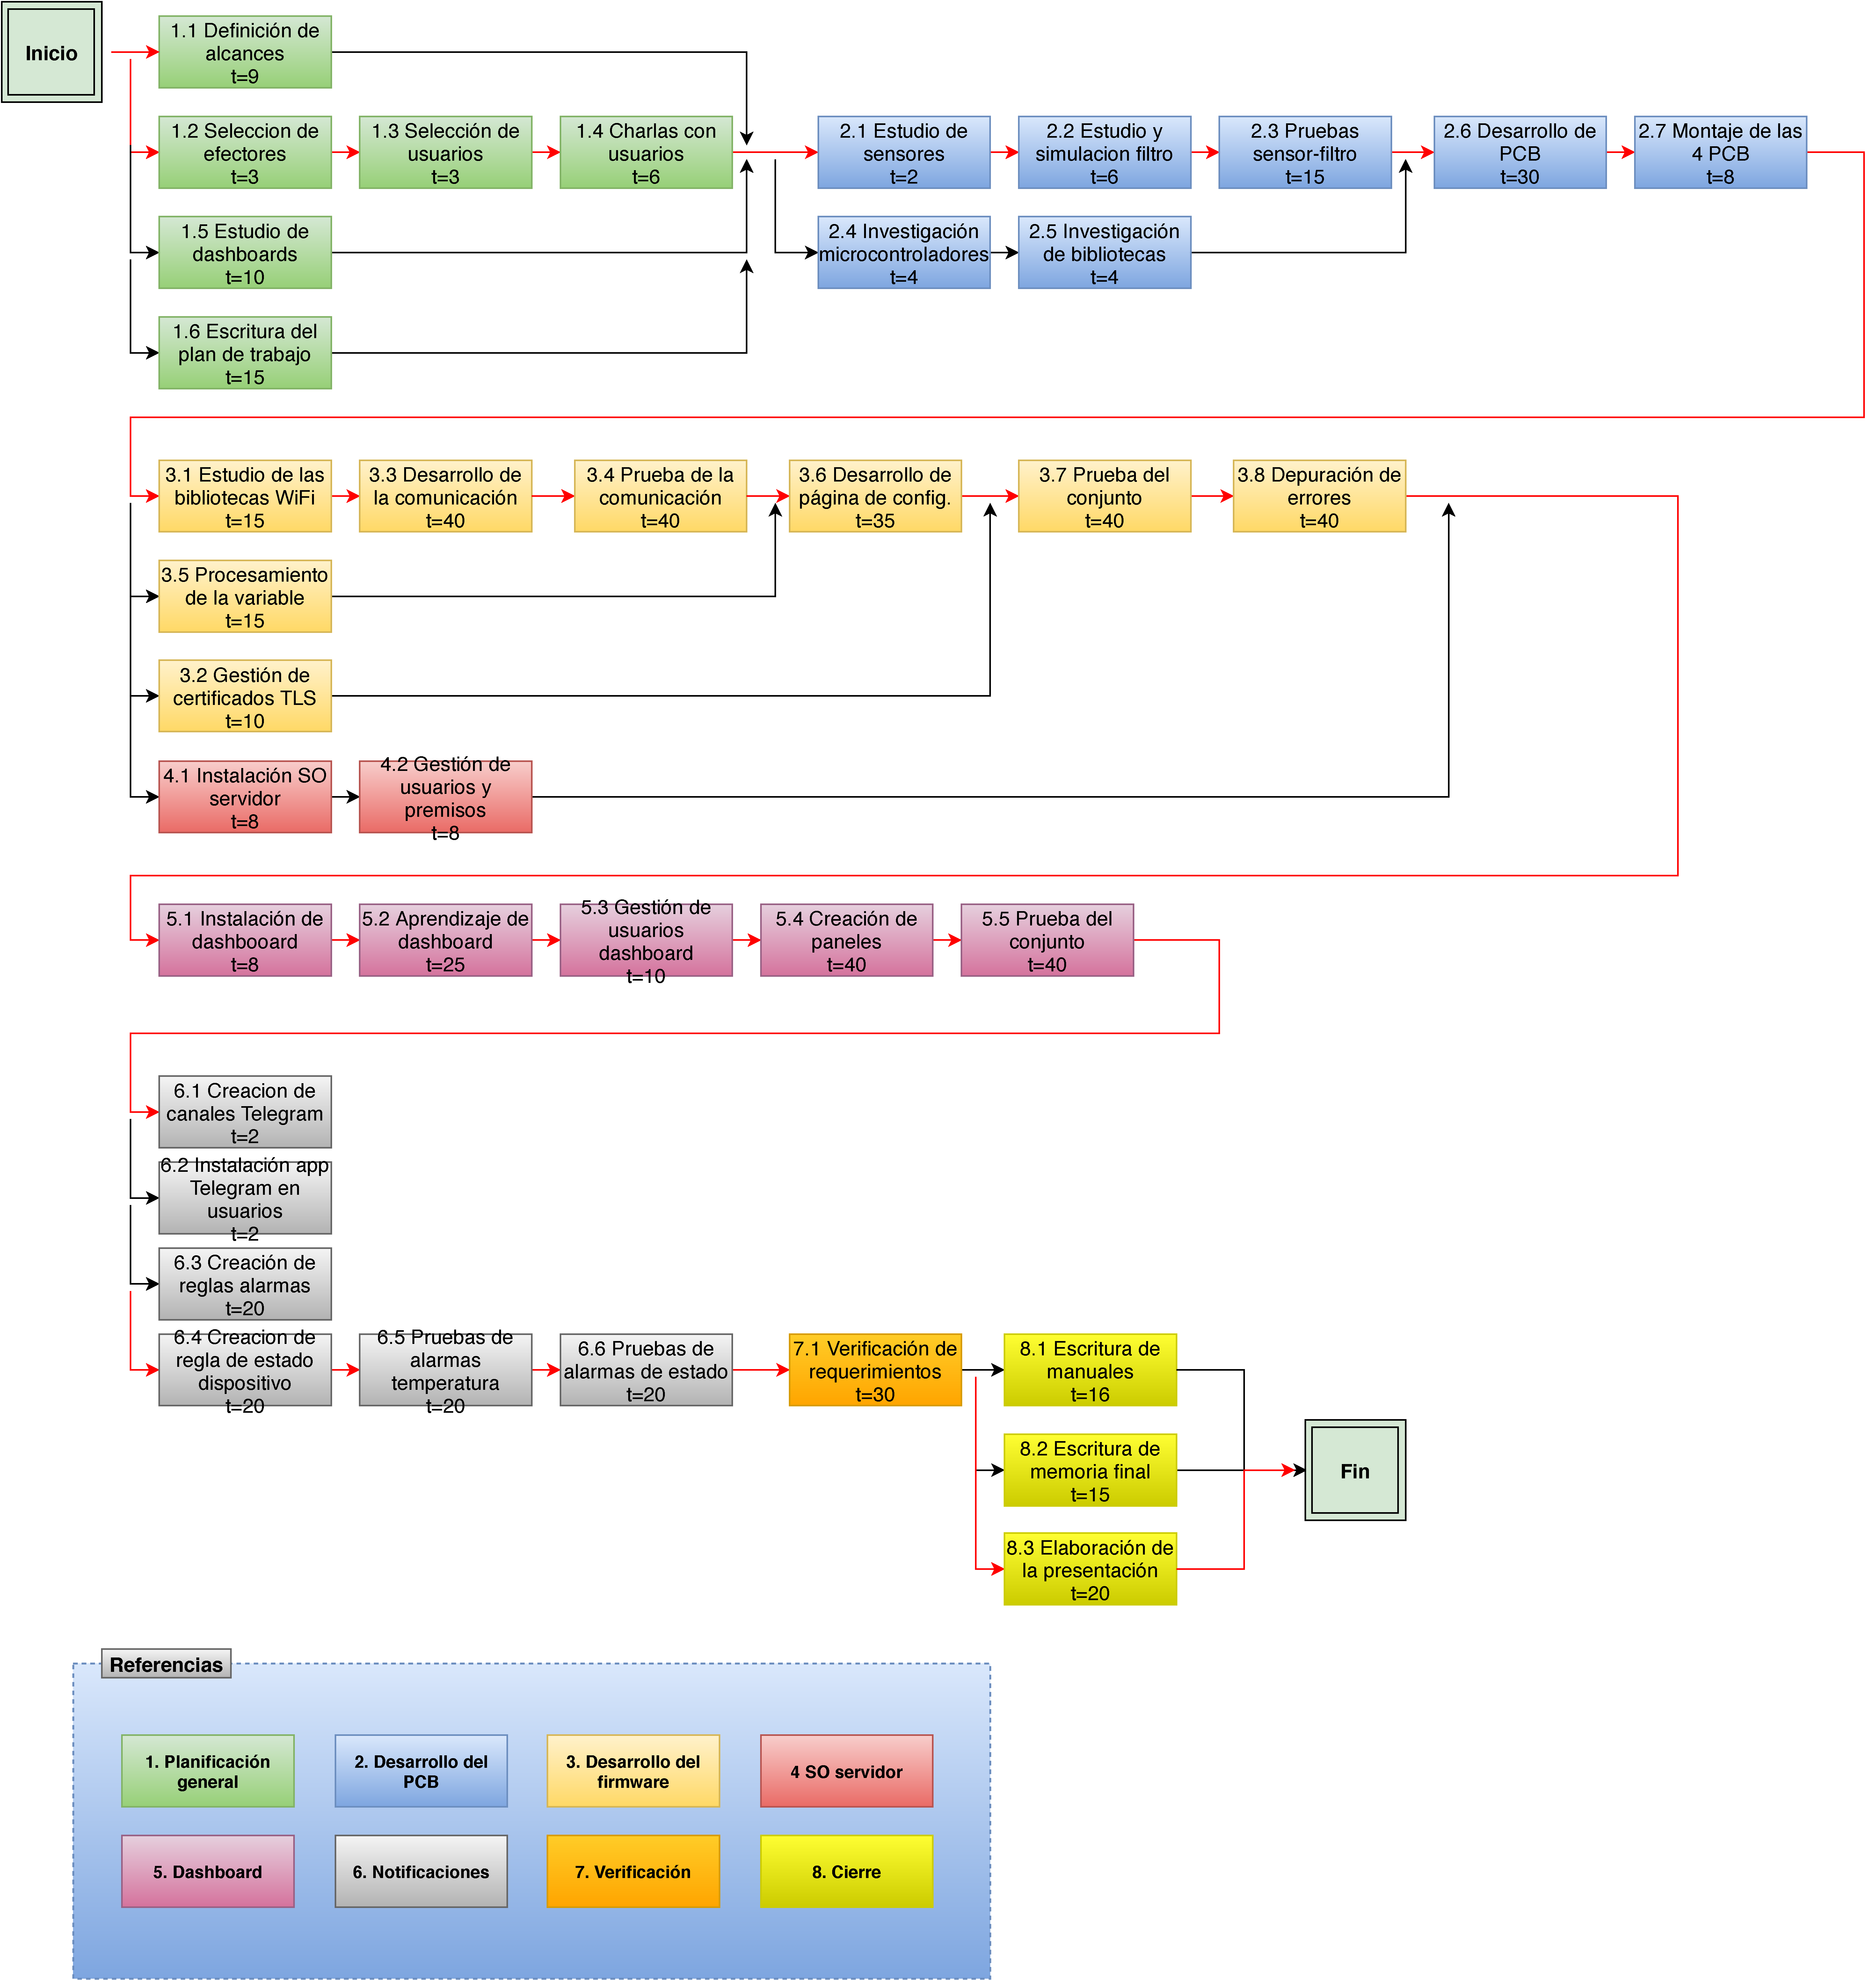
\includegraphics[width=1\textwidth]{./Figuras/act_on_node_1.pdf}
\caption{Diagrama \textit{Activity on Node}}
\label{fig:AoN}
\end{figure}



%Indicar claramente en qué unidades están expresados los tiempos.
%De ser necesario indicar los caminos semicríticos y analizar sus tiempos mediante un cuadro.
%Es recomendable usar colores y un cuadro indicativo describiendo qué representa cada color, como se muestra en el siguiente ejemplo:



\section{8. Diagrama de Gantt}
\label{sec:gantt}

En la figura \ref{wbs} se aprecia la tabla del desglose de actividades con sus fechas de inicio y fin, duración y tareas predecesoras.

%Pegar acá una captura de pantalla del diagrama de Gantt, cuidando que la letra sea suficientemente grande como para ser legible. 
%Si el diagrama queda demasiado ancho, se puede pegar primero la ``tabla'' del Gantt y luego pegar la parte del diagrama de barras del diagrama de Gantt.


\begin{figure}[htpb]
\centering 
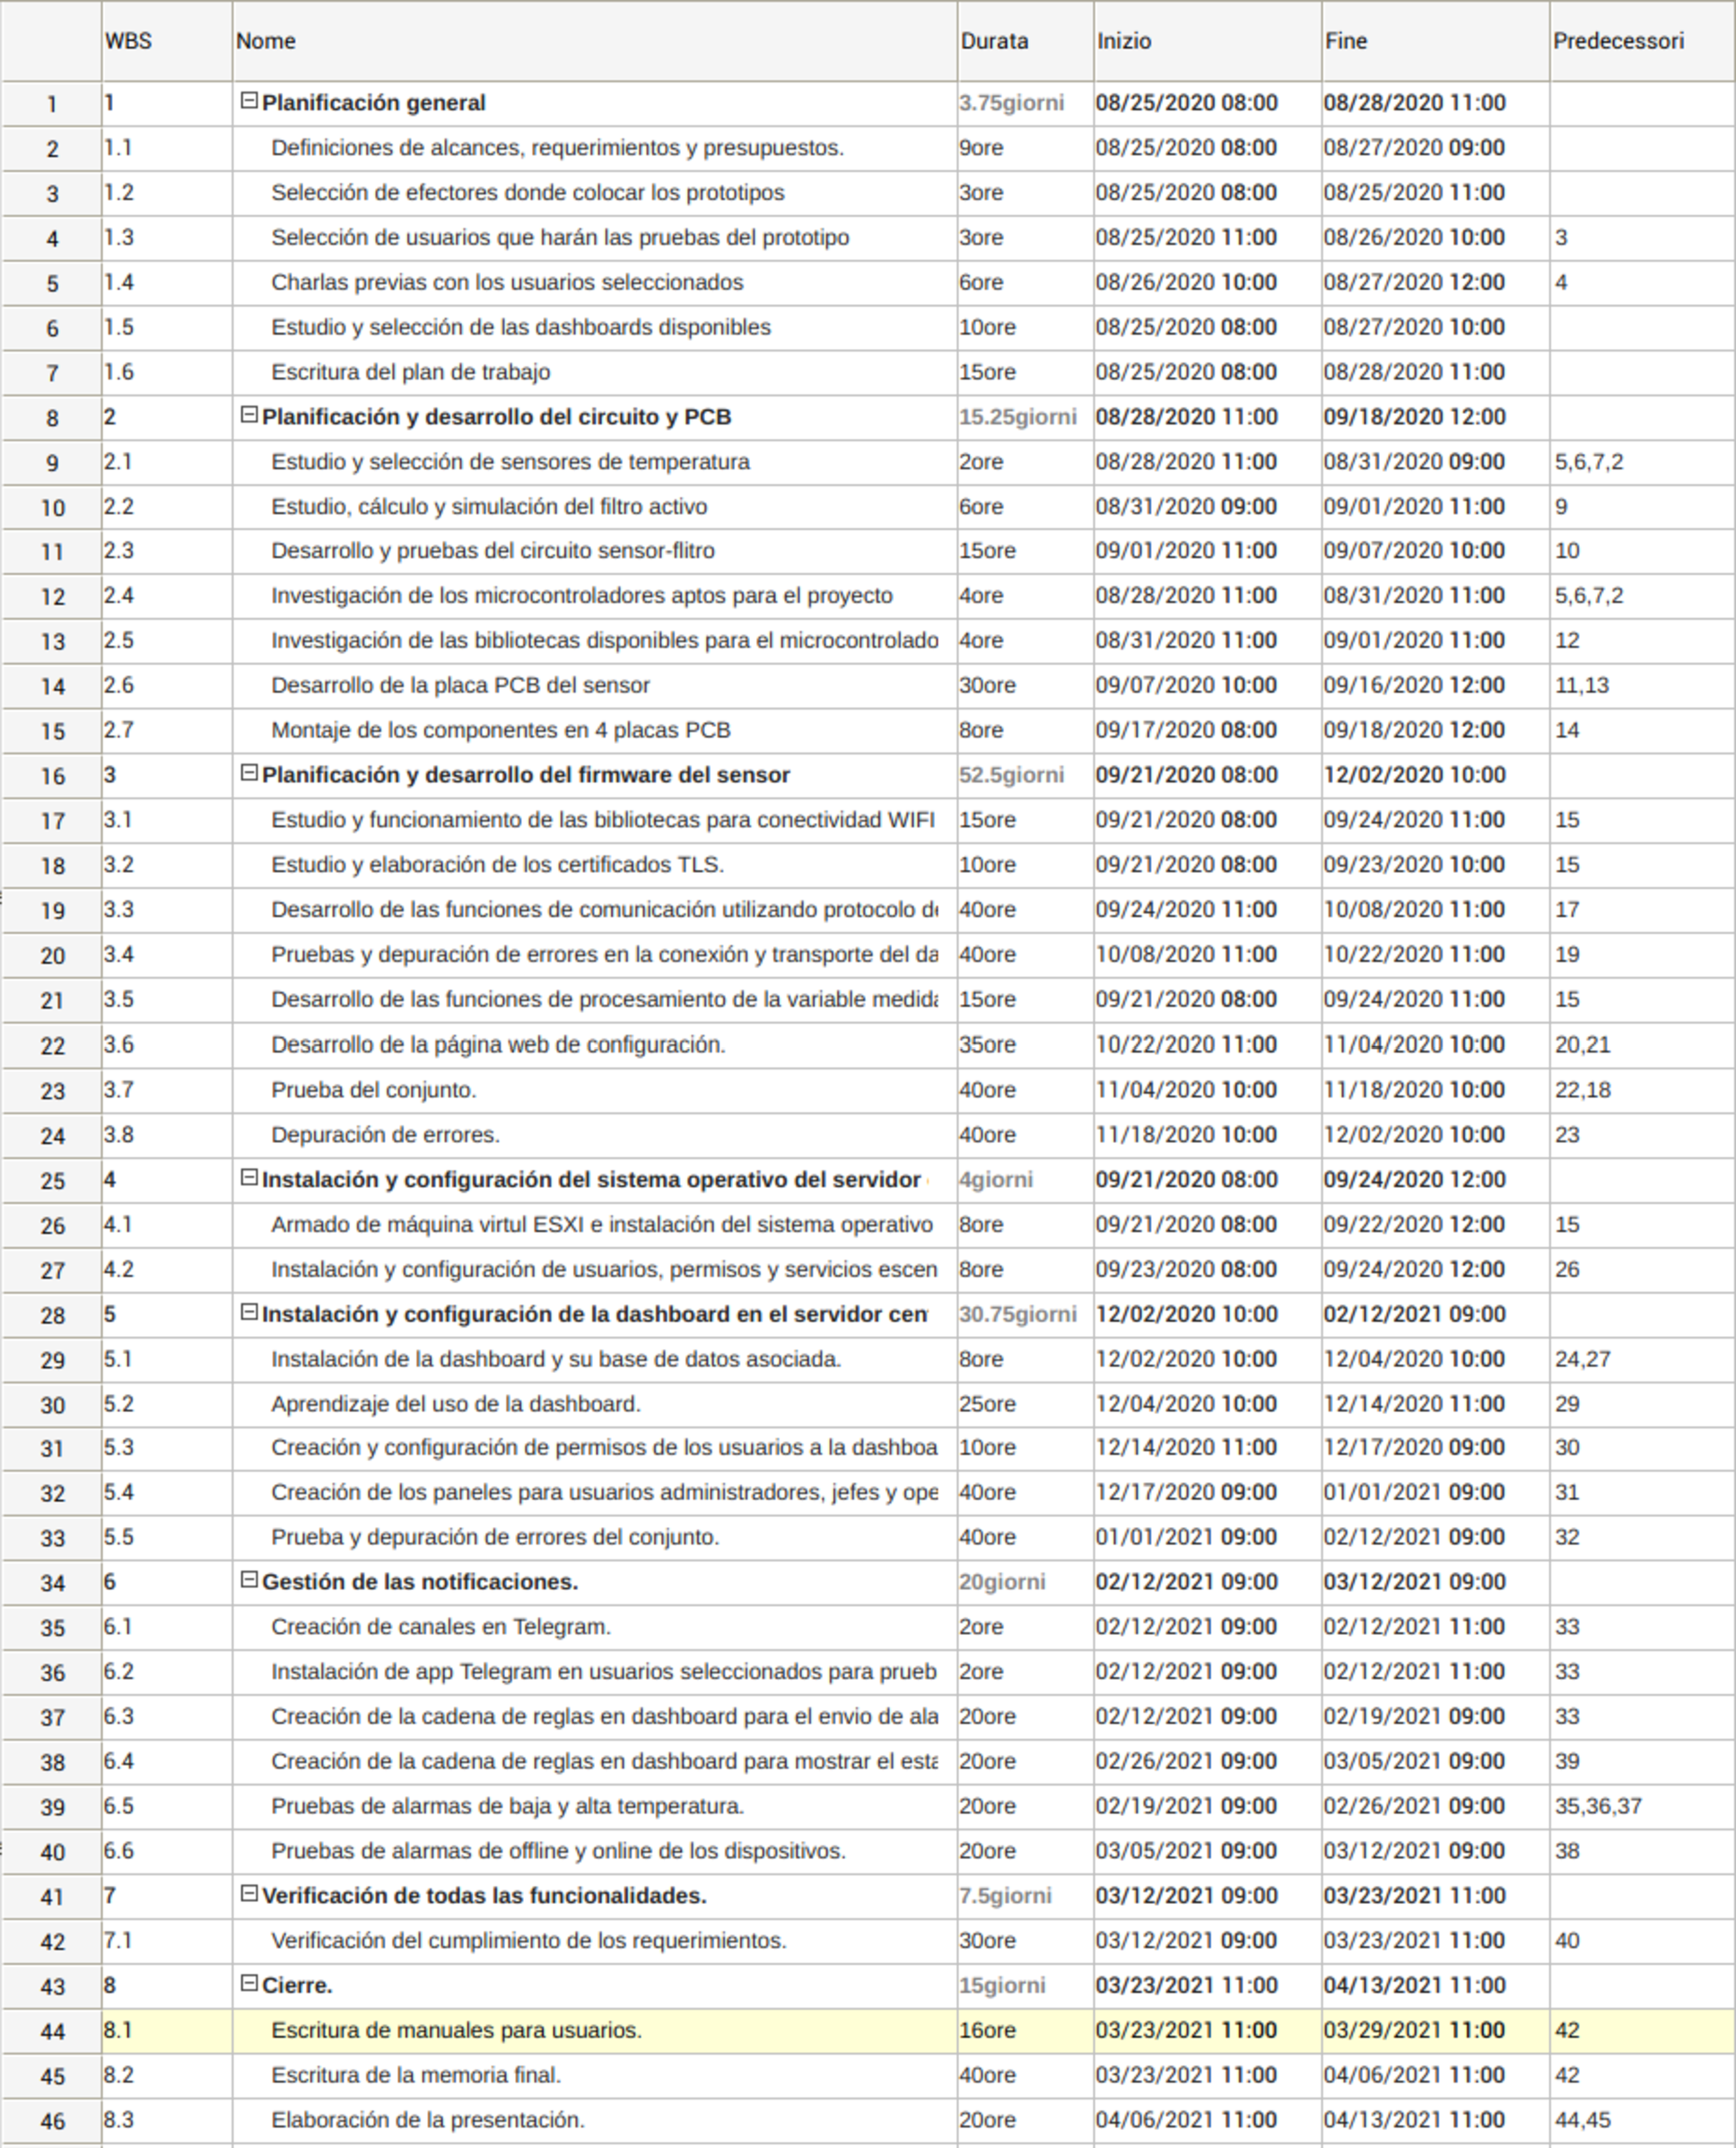
\includegraphics[width=1\textwidth]{./Figuras/wbs.pdf}
\caption{\textit{Tabla de actividades}}
\label{wbs}
\end{figure}



%Configurar el software para que en la parte de la tabla muestre los códigos del EDT (WBS).\\
%Configurar el software para que al lado de cada barra muestre el nombre de cada tarea.\\
%Revisar que la fecha de finalización coincida con lo indicado en el Acta Constitutiva.

En las figuras \ref{gantt1} y \ref{gantt2} se observa el diagrama de gantt.
Para la elaboración del mismo, se tomó una jornada de trabajo de 4 horas diarias y se ajustó el calendario para exceptuar el mes de enero de 2021.

\begin{landscape}
\begin{figure}[htpb]
\centering 
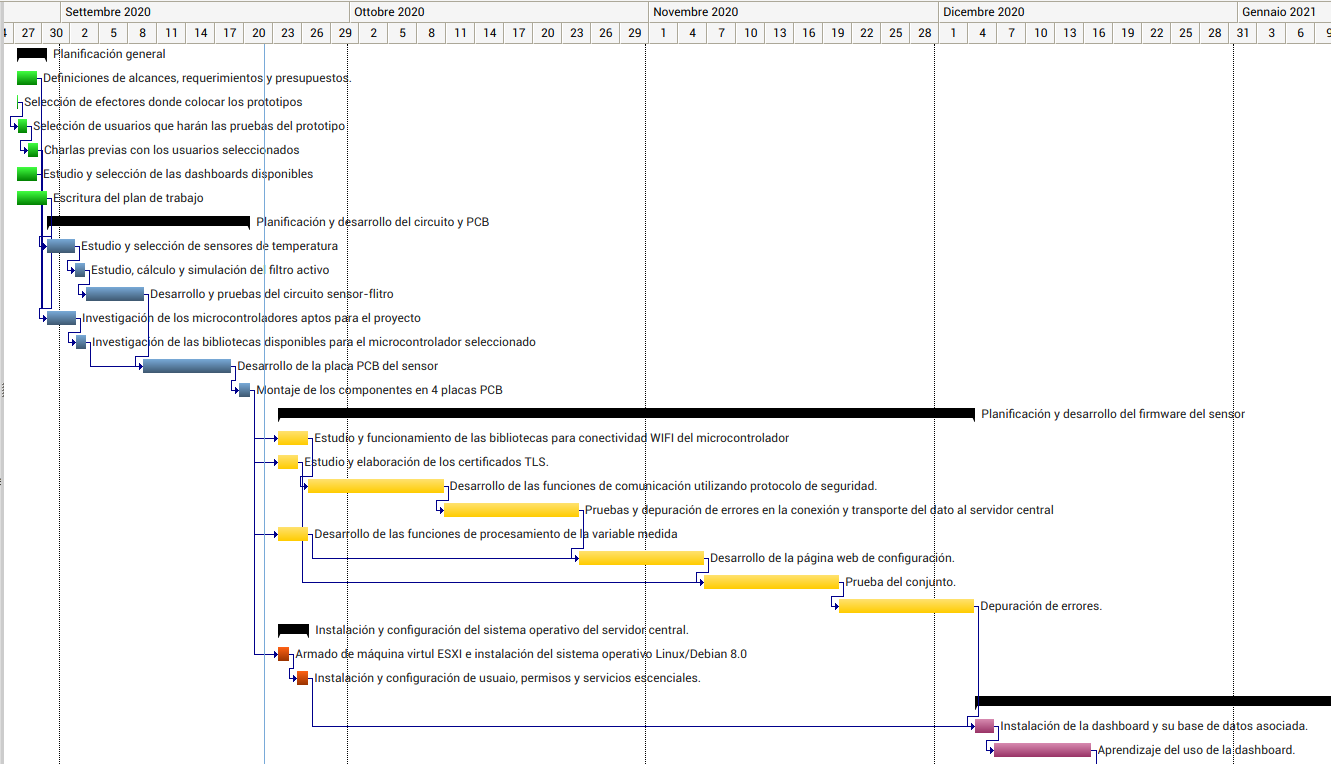
\includegraphics[width=1.5\textwidth]{./Figuras/gantt1.png}
\vspace{-0.3cm} 
\caption{\textit{Diagrama de gantt parte 1/2}}
\label{gantt1}
\end{figure}
\end{landscape}

\begin{landscape}
\begin{figure}[htpb]
\centering 
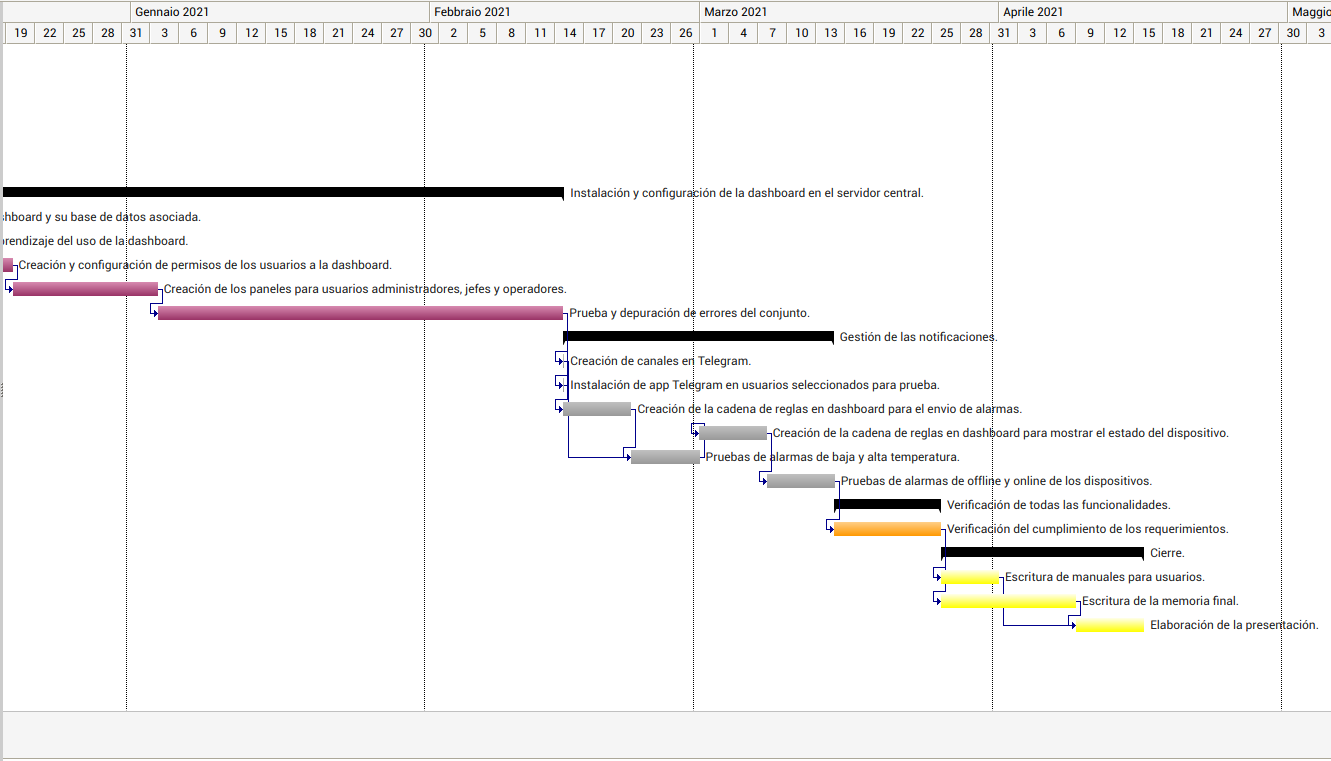
\includegraphics[width=1.5\textwidth]{./Figuras/gantt2.png}
\vspace{-0.3cm} 
\caption{\textit{Diagrama de gantt parte 2/2}}
\label{gantt2}
\end{figure}
 \end{landscape}



\section{9. Matriz de uso de recursos de materiales}
\label{sec:recursos}
En la tabla \ref{recursos1}, se visualiza la utilización de los recursos. Las cantidades están expresadas en horas.

Descripción de los recursos necesarios.

PC desktop: será una computadora de escritorio con sistema operativo Ubuntu 20.04 con las utilidades de oficina instaladas.
\begin{itemize}
\item Texmaker
\item LibreOffice.
\item Chrome con extensión Gantter.
\item Git.
\end{itemize}

Laboratorio: estará compuesto por herramientas e instrumental para desarrollo y armado de placas electrónicas.
\begin{itemize}
\item Osciloscopio.
\item Estación de soldadura/desoldadura.
\item Generador de ondas arbitrarias.
\item Fuente de alimentación.
\item Multímetro de banco.
\item PC de desarrollo con las utilidades requeridas, Visual Studio Code, Matlab, Git.
\item Módulos nodeMCU con microcontroladores ESP8266.
\item Red WiFi con permisos de administración.
\end{itemize}

Servidor: un hardware de servidor donde se instalará la dashboard. Deberá poseer al menos 4 Gb de memoria RAM y capacidad de almacenamiento en disco rígido de al menos 30 Gb. 

Sala de reuniones: espacio de trabajo para albergar al menos un grupo de 10 personas, deberá poseer pantalla y computadora con conexión a Internet.

Teléfono móvil: un teléfono propio para hacer las pruebas de recepción de alarmas.

\begin{table}

\centering
\resizebox{\textwidth}{!}{
\begin{tabular}{|c|c|c|c|c|c|c|}
%\begin{tabularx}{\linewidth}{@{}|c|X|X|X|X|X|c|@{}}
\hline
\cellcolor[HTML]{C0C0C0} & \cellcolor[HTML]{C0C0C0} & \multicolumn{5}{c|}{\cellcolor[HTML]{C0C0C0}Recursos requeridos (horas)} \\ \cline{3-7} 
\multirow{-2}{*}{\cellcolor[HTML]{C0C0C0}\begin{tabular}[c]{@{}c@{}}Código\\ WBS\end{tabular}} & \multirow{-2}{*}{\cellcolor[HTML]{C0C0C0}\begin{tabular}[c]{@{}c@{}}Nombre \\ tarea\end{tabular}} & PC desktop & Laboratorio & Servidor & Sala reuniones & Teléfono móvil \\ \hline
 
 1.1&Definición de alcances & 9 & &  &  &  \\ \hline
 1.2&Selección de efectores &  &  &  & 3 &  \\ \hline
 1.3&Selección de usuarios  &  &  &  & 3 &\\ \hline
 1.4&Charlas con usuarios  &  &  &  & 6 &\\ \hline
 1.5&Estudio de dashboards & 10 &  &  &  &\\ \hline
 1.6&Escritura del plan de trabajo & 15 &  &  &  &\\ \hline
 2.1&Estudio de sensores  & 2 &  &  &  &\\ \hline
 2.2&Estudio y simulación filtro  &  & 6 &  &  &\\ \hline 
 2.3&Pruebas sensor filtro  &  & 15 &  &  &\\ \hline
 2.4&Investigación microcontroladores  & 4 &  &  &  &\\ \hline
 2.5&Investigación bibliotecas  & 4 &  &  &  &\\ \hline
 2.6&Desarrollo PCB  &  & 30 &  &  &\\ \hline
 2.7&Montaje PCB  &  & 8 &  &  &\\ \hline
  3.1&Estudio bibliotecas WiFi & 15 &  &  &  &\\ \hline
 3.2&Gestión de certificados TLS  & 10 &  &  &  &\\ \hline
 3.3&Desarrollo comunicación  &  & 40 &  &  &\\ \hline
 3.4&Prueba comunicación  &  & 40 &  &  &\\ \hline
 3.5&Procesamiento variable  &  & 15 &  &  &\\ \hline
 3.6&Desarrollo página configuración &  & 35 &  &  &\\ \hline
 3.7&Prueba del conjunto  &  & 40 &  &  &\\ \hline
 3.8&Depuración de errores  &  & 40 &  &  &\\ \hline
 4.1&Instalación SO servidor  &  &  & 8 &  &\\ \hline
 4.2&Gestión de usuarios y permisos &  &  & 8 &  &\\ \hline
 5.1&Instalación dashboard  & 4 &  & 4 &  &\\ \hline 
 5.2&Aprendizaje uso dashboard  & 15 &  & 10 &  &\\ \hline
 5.3&Gestión usuarios dashboard  & 5 &  & 5 &  &\\ \hline
 5.4&Creación de paneles  & 20 &  & 20 &  &\\ \hline
 5.5&Prueba del conjunto  & 20 &  & 20 &  &\\ \hline
  6.1&Creación canales Telegram  & 2 &  &  &  &\\ \hline
 6.2&Instalación app Telegram &  &  &  &  &2\\ \hline
 6.3&Creación reglas de alarmas & 10 &  & 10 &  &\\ \hline
 6.4&Creación reglas de estado &  10 &  & 10 &  &\\ \hline
 6.5&Prueba alarma temperatura & 15 &  &  &  &5\\ \hline
 6.6&Prueba alarma estado & 15 &  &  &  &5\\ \hline
 7.1&Verificación de requerimientos & 20  &  &5  &  &5\\ \hline
 8.1&Escritura de manuales & 16 &  &  &  &\\ \hline
 8.2&Escritura de memoria final & 40 &  &  &  &\\ \hline
 8.3&Elaboración de la presentación & 20 &  &  &  &\\ \hline
 \end{tabular}%
 }
 \caption{\textit{Tabla de asignación de recursos}}
 \label{recursos1}
 \end{table}
 
\section{10. Presupuesto detallado del proyecto}
\label{sec:presupuesto}

\begin{table}[htpb]
\centering
\begin{tabularx}{\linewidth}{@{}|X|c|r|r|@{}}
\hline
\rowcolor[HTML]{C0C0C0} 
\multicolumn{4}{|c|}{\cellcolor[HTML]{C0C0C0}COSTOS DIRECTOS} \\ \hline
\rowcolor[HTML]{C0C0C0} 
Descripción &
  \multicolumn{1}{c|}{\cellcolor[HTML]{C0C0C0}Cantidad} &
  \multicolumn{1}{c|}{\cellcolor[HTML]{C0C0C0}Valor unitario} &
  \multicolumn{1}{c|}{\cellcolor[HTML]{C0C0C0}Valor total} \\ \hline

 Horas de ingeniería &
  \multicolumn{1}{c|}{663} &
  \multicolumn{1}{c|}{800} &
  \multicolumn{1}{c|}{530400} \\ \hline

 Fabricación de PCB&
  \multicolumn{1}{c|}{10} &
  \multicolumn{1}{c|}{800} &
  \multicolumn{1}{c|}{8000} \\ \hline

 Componentes electrónicos para un nodo&
  \multicolumn{1}{c|}{10} &
  \multicolumn{1}{c|}{1500} &
  \multicolumn{1}{c|}{15000} \\ \hline
 
 Cables y conectores&
  \multicolumn{1}{c|}{1} &
  \multicolumn{1}{c|}{4500} &
  \multicolumn{1}{c|}{4500} \\ \hline  
  
 Cajas plásticas&
  \multicolumn{1}{c|}{10} &
  \multicolumn{1}{c|}{300} &
  \multicolumn{1}{c|}{3000} \\ \hline

 Estaño 60/40 250gr&
  \multicolumn{1}{c|}{1} &
  \multicolumn{1}{c|}{1500} &
  \multicolumn{1}{c|}{1500} \\ \hline

\multicolumn{3}{|c|}{SUBTOTAL} &
  \multicolumn{1}{c|}{562400} \\ \hline
\rowcolor[HTML]{C0C0C0} 
\multicolumn{4}{|c|}{\cellcolor[HTML]{C0C0C0}COSTOS INDIRECTOS} \\ \hline
\rowcolor[HTML]{C0C0C0} 
Descripción &
  \multicolumn{1}{c|}{\cellcolor[HTML]{C0C0C0}Cantidad} &
  \multicolumn{1}{c|}{\cellcolor[HTML]{C0C0C0}Valor unitario} &
  \multicolumn{1}{c|}{\cellcolor[HTML]{C0C0C0}Valor total} \\ \hline
  
\multicolumn{1}{|l|}{30 \% de los costos directos} &
  \multicolumn{1}{c|}{1} &
  \multicolumn{1}{c|}{168720} &
  \multicolumn{1}{c|}{168720} \\ \hline

\multicolumn{3}{|c|}{SUBTOTAL} &
  \multicolumn{1}{c|}{168720} \\ \hline
\rowcolor[HTML]{C0C0C0}
\multicolumn{3}{|c|}{TOTAL} &
\multicolumn{1}{c|}{731120}   \\ \hline
\end{tabularx}%
\end{table}


\section{11. Matriz de asignación de responsabilidades}
\label{sec:responsabilidades}
%\begin{consigna}{red}
%Establecer la matriz de asignación de responsabilidades y el manejo de la autoridad completando la siguiente tabla:
En el cuadro \ref{tab:resp} se muestra la matriz de asignación de responsabilidades y el manejo de la autoridad.
\begin{table}[htpb]

\centering
\resizebox{\textwidth}{!}{%
\begin{tabular}{|c|c|c|c|c|c|}
\hline
\rowcolor[HTML]{C0C0C0} 
\cellcolor[HTML]{C0C0C0} &
  \cellcolor[HTML]{C0C0C0} &
  \multicolumn{4}{c|}{\cellcolor[HTML]{C0C0C0}Listar todos los nombres y roles del proyecto} \\ \cline{3-6} 
\rowcolor[HTML]{C0C0C0} 
\cellcolor[HTML]{C0C0C0} &
  \cellcolor[HTML]{C0C0C0} &
  Responsable &
  Director &
  Impulsor &
  Cliente \\ \cline{3-6} 
\rowcolor[HTML]{C0C0C0} 
\multirow{-3}{*}{\cellcolor[HTML]{C0C0C0}\begin{tabular}[c]{@{}c@{}}Código\\ WBS\end{tabular}} &
  \multirow{-3}{*}{\cellcolor[HTML]{C0C0C0}Nombre de la tarea} &
  \authorname &
  \supname &
  Roberto Collelo &
  \clientename \\ \hline
 1.1&Definición de alcances & P & A &  & A \\ \hline
 1.2&Selección de efectores &  S & I &  & A  \\ \hline
 1.3&Selección de usuarios  &  S & I &  & A\\ \hline
 1.4&Charlas con usuarios  & P  & I &  & I\\ \hline
 1.5&Estudio de dashboards & P & I &  & \\ \hline
 1.6&Escritura del plan de trabajo & P & A  &  & I \\ \hline
 2.1&Estudio de sensores  & P &  & C  & \\ \hline
 2.2&Estudio y simulación filtro  & P  & C &  &\\ \hline 
 2.3&Pruebas sensor filtro  &  P & A &  & \\ \hline
 2.4&Investigación microcontroladores  & P  & I & C &\\ \hline
 2.5&Investigación bibliotecas  & P  & I & C &\\ \hline
 2.6&Desarrollo PCB  & P  & I & C &\\ \hline
 2.7&Montaje PCB  & P  & A &  & I\\ \hline
 3.1&Estudio bibliotecas WiFi  & P & I & C &\\ \hline
 3.2&Gestión de certificados TLS  & P &  &  &\\ \hline
 3.3&Desarrollo comunicación  & P & I &  &\\ \hline
 3.4&Prueba comunicación  & P & A &  & I\\ \hline
 3.5&Procesamiento variable  & P  & I & C &\\ \hline
 3.6&Desarrollo página configuración & P  & I & C &\\ \hline
 3.7&Prueba del conjunto  & P & A &  & A\\ \hline
 3.8&Depuración de errores  & P & A &  &\\ \hline
 4.1&Instalación SO servidor  & P & I &  &\\ \hline
 4.2&Gestión de usuarios y permisos & P & I &  &\\ \hline
 5.1&Instalación dashboard  & P & I &  &\\ \hline 
 5.2&Aprendizaje uso dashboard  & P & I &  &\\ \hline
 5.3&Gestión usuarios dashboard  & P & I &  &\\ \hline
 5.4&Creación de paneles  & P & C & C & C\\ \hline
 5.5&Prueba del conjunto  & P & A &  & A\\ \hline
 6.1&Creación canales Telegram  & P & I &  &\\ \hline
 6.2&Instalación app Telegram & S & I &  &  \\ \hline
 6.3&Creación reglas de alarmas & P & I &  &\\ \hline
 6.4&Creación reglas de estado & P & I &  &\\ \hline
 6.5&Prueba alarma temperatura & P & A &  & I\\ \hline
 6.6&Prueba alarma estado & P & A &  & I \\ \hline
 7.1&Verificación de requerimientos & P & A &  & A\\ \hline
 8.1&Escritura de manuales & P & A & C & I\\ \hline
 8.2&Escritura de memoria final & P & A &  & I\\ \hline
 8.3&Elaboración de la presentación & P & A &  & I\\ \hline

\end{tabular}%
}
\vspace{.5cm}
\caption{\textit{Matriz de asignación de responsabilidades}}
\label{tab:resp}
\end{table}

{\footnotesize
Referencias:
\begin{itemize}
	\item P = Responsabilidad Primaria
	\item S = Responsabilidad Secundaria
	\item A = Aprobación
	\item I = Informado
	\item C = Consultado
\end{itemize}
} %footnotesize

%Una de las columnas debe ser para el Director, ya que se supone que participará en el proyecto.
%A su vez se debe cuidar que no queden muchas tareas seguidas sin ``A'' o ``I''.

%Importante: es redundante poner ``I/A'' o ``I/C'', porque para aprobarlo o responder consultas primero la persona debe ser informada.

%\end{consigna}

\section{12. Gestión de riesgos}
\label{sec:riesgos}
Se describen los riesgos para el desarrollo del proyecto y su plan de mitigación.

\textbf{a) Identificación de los riesgos y estimación de sus consecuencias:}
 
Riesgo 1: El panel de control seleccionado no cubre las necesidades básicas. Si el sistema de visualización, no permite configurar la estructura jerárquica geográfica o no posee la capacidad de generar roles para distintos usuarios, se deberá optar por otra solución, lo que atrasará de manera grave el proyecto.
\begin{itemize}
\item Severidad (S): 8. El riesgo es alto, ya que no podremos cumplir con los requerimientos del cliente.
\item Ocurrencia (O): 3. Si se verifican los requerimientos del cliente, la ocurrencia de este riesgo será baja. Para ello se debe invertir un tiempo razonable en el estudio de las soluciones disponibles.
\end{itemize}   

Riesgo 2: Error en el diseño del circuito electrónico. Implicaría indefectiblemente un error en el diseño del PCB.
\begin{itemize}
\item Severidad (S): 10. Muy severo ya produciría un mal funcionamiento. 
\item Ocurrencia (O): 4. Se asigna esta ocurrencia ya que se harán las pruebas necesarias para depurar los errores.
\end{itemize}

Riesgo 3: Error en la elección del microcontrolador. Es grave si el error es inherente a la capacidad de RAM o la capacidad de la memoria de programa.
\begin{itemize}
\item Severidad (S): 3. Se da este valor al asegurar que posea todos los recursos físicos suficientes.
\item Ocurrencia (O): 1. Se verificará que el dispositivo tenga suficientes recursos para el desarrollo de la aplicación.
\end{itemize}

Riesgo 4: Falla del firmware. Fallas reiteradas en el firmware del nodo, ocasionará un atraso en la ejecución del proyecto, por lo que se deberá tener muy en cuenta al hacer su desarrollo. 
\begin{itemize}
\item Severidad (S): 7. Un error de este tipo causará un funcionamiento inestable o no fiable del sistema.
\item Ocurrencia (O): 7. Se considera este número debido a la dificultad en el desarrollo del firmware.
\end{itemize}

Riesgo 5: Atraso en la fabricación del PCB. Se preve que la fabricación sea derivada a un proveedor externo al país. Si bien no se tiene conocimiento de atrasos en la entrega, al ser un artículo importado, requiere de una previsión por un eventual cambio en las reglas de importación.
\begin{itemize}
\item Severidad (S): 10. Se considera muy grave, ya que no podrá seguir adelante el proyecto
\item Ocurrencia (O): 5. Se asigna este valor ya que la compra del producto depende de su importación.
\end{itemize}

Riesgo 6: Error en el diseño del PCB. Se confiará la fabricación del PCB a un proveedor que haga una evaluación primaria del diseño, esto permite descubrir errores groseros y solucionarlos antes de su fabricación.
\begin{itemize}
\item Severidad (S): 4. Puede ser grave si el error se propaga a todos los componentes del circuito (falla en las pistas de alimentación o errores groseros).
\item Ocurrencia (O): 4. Se asigna esta probabilidad ya que es bastante común alguna falla en el diseño pero que resulta de sencilla resolución.
\end{itemize}


\textbf{b) Tabla de gestión de riesgos:}

\begin{table}[htpb]
\centering
\begin{tabularx}{\linewidth}{@{}|X|c|c|c|c|c|c|@{}}
\hline
\rowcolor[HTML]{C0C0C0} 
Riesgo & S & O & RPN & S* & O* & RPN* \\ \hline
1 & 8  & 3  &  \cellcolor[HTML]{7ab560}24   &   - &  -  &    -  \\ \hline
2 &  10 &  4 & \cellcolor[HTML]{c94848} 40  &  9  &  1  &  \cellcolor[HTML]{7ab560}9 \\ \hline
3 &  3 & 1  &   \cellcolor[HTML]{7ab560}3  &  -  &  -  &    -  \\ \hline
4 & 7  & 7  &  \cellcolor[HTML]{c94848}49   &  9  & 3   & \cellcolor[HTML]{7ab560}27  \\ \hline
5 &  10 &  5 &  \cellcolor[HTML]{c94848}50   &  4  & 4   & \cellcolor[HTML]{7ab560}16  \\ \hline
6 & 4  & 4  &   \cellcolor[HTML]{7ab560}16  &  -  &  - &   - \\ \hline
\end{tabularx}%
\end{table}

Criterio adoptado: 
Se tomarán medidas de mitigación en los riesgos cuyos números de RPN sean igual o mayores a 35

Nota: los valores marcados con (*) en la tabla corresponden luego de haber aplicado la mitigación.

\textbf{c) Plan de mitigación de los riesgos que originalmente excedían el RPN máximo establecido:}
 
 Se trabajará en un plan de mitigación para los riesog 2, 4 y 5, ya que exceden el valor máximo admitido: 35.
 
Riesgo 2: Se trabajará utilizado una placa de armado de prototipos. Luego se pasará a una placa PCB intermedia realizada en forma casera, con la ventaja de tener todos los componentes electrónicos soldados a la misma, evitando así los falsos contactos tan comunes en las placas prototipo.
\begin{itemize}
\item Severidad (S): 9. No se modifica
\item Probabilidad de ocurrencia (O): 1. Se espera que con la aplicación de este plan, el riesgo disminuya sustancialmente.
\end{itemize}

Riesgo 4: Se trabajará sobre la prueba y depuración de cada uno de los módulos de software que intervienen. Se pondrá el sistema a prueba durante un tiempo razonable hasta lograr la estabilidad. Durante este tiempo se harán los modificaciones necesarias.
\begin{itemize}
\item Severidad (S): 9. No se modifica
\item Probabilidad de ocurrencia (O): 3. Haciendo depuraciones y pruebas exhaustivas, se espera una baja probabilidad de fallas.
\end{itemize}

Riesgo 5:  Se tratará de tener  proveedores locales sustitutos aunque represente un aumento en los costos finales. 
\begin{itemize}
\item Severidad (S): 4. Con proveedores locales, no hay proceso de importación. Sólo puede haber demoras en la fabricación.
\item Probabilidad de ocurrencia (O): 4. Si no es posible la importación, se espera que los proveedores locales entreguen el trabajo a tiempo.
\end{itemize}



\section{13. Gestión de la calidad}
\label{sec:calidad}


Se presentan a continuación los requerimientos con sus verificaciones y validaciones.

\begin{itemize} 
\item Req 1.1: Cada nodo estará compuesto por un microcontrolador un elemento sensor de
temperatura y la electrónica asociada para su funcionamiento.
	\begin{itemize}
	\item Verificación: se observará si el diagrama esquemático del circuito incorpora un microcontrolador y un sensor de temperatura.
	\item Validación: Se comprobará si la página web interna muestra la inclusión de un microcontrolador y un sensor de temperatura.
\end{itemize}

\item 1.2: El microcontrolador utilizado deberá estar en fase de producción activa.
\begin{itemize}
\item Verificación: se observará la información que figura en la página web del fabricante del microcontrolador seleccionado.
\item Validación: al comprar el dispositivo, el proveedor indica el estado de fabricación.
\end{itemize}

\item 1.3 El microcontrolador deberá contener capa física WiFi.

\begin{itemize}
\item Verificación: se observará la hoja de datos del componente.
\item Validación: se graba un programa de ejemplo para comprobar la conexión WiFi exitosa.
\end{itemize}


\item 1.4 El elemento sensor deberá tener un rango de medición entre -50 y 100 ºC
\begin{itemize}
\item Verificación: se observará la hoja de datos del sensor.
\item Validación: se hará una prueba de funcionamiento a temperaturas entre -50 y 100 para observar que los valores medidos sean los valores esperados.
\end{itemize}


\item 1.5 El nodo deberá incluir en su circuito un filtro activo de 2º orden para la filtrar las componentes de alta frecuencia de la entrada de temperatura.
\begin{itemize}
\item Verificación: se observará en el diagrama esquemático del circuito la incorporación de un operacional dispuesto como filtro activo de segundo orden en la entrada analógica del microcontrolador. Se harán simulaciones introduciendo ruido para valorar el desempeño de este circuito.
\item Validación: se harán pruebas con generador de ondas arbitrarias, introduciendo ruido en la entrada analógica, para comprobar la efectividad del filtro.
\end{itemize}

\item 1.6 El nodo deberá incorporar indicadores luminosos de conexión con la red WiFi, conexión con el servidor central e indicador de fuera de rango de temperatura.

\begin{itemize}
\item Verificación: se observará en el diagrama esquemático del circuito la incorporación de tres leds: conexión WiFi, Fuera de rango y conexión con servidor central.
\item Validación: se harán pruebas de conexión, desconexión de la red WiFi y del servidor central para validar el funcionamiento. Se simulará a través de la inyección de una tensión equivalente en la entrada analógica el funcionamiento del led de fuera de rango.
\end{itemize}

\item 2.1 Deberá contener un conjunto de parámetros que identifiquen de forma unívoca el sensor dentro del sistema.
\item 2.2 Los parámetros se deberán almacenar en memoria no volátil.


\begin{itemize}
\item Verificación: se inspeccionará el código fuente del firmware para observar la inclusión de tales parámetros y su grabación en memoria no volátil.
\item Validación: a través de la página web del dispositivo se comprobará que existan los parámetros. Se procederá al cambio de valores, reinicio del dispositivo y comprobación del cambio de los parámetros antes grabados.
\end{itemize}

\item 2.3 Deberá gestionar el procesamiento de los valores de temperatura: muestreo cada segundo y promediado cada 600 segundos.
\begin{itemize}
\item Verificación: se inspeccionará el código fuente del firmware para observar la inclusión del algoritmo de muestreo y promedio de la temperatura.
\item Validación: a través de la página web del dispositivo se comprobará que se actualice una medición cada 10 minutos.
\end{itemize}

\item 2.4 Deberá incluir parámetros de calibración como offset y ganancia para su futuro contraste con un instrumento patrón.
\item 2.7 Deberá ser capaz de conectar distintos modelos de sensores de temperatura.
\begin{itemize}
\item Verificación: se inspeccionará el código fuente del firmware para observar la inclusión los parámetros que definan una función de transferencia que sirva para caracterizar cualquier sensor que se utilice.
\item Validación: a través de la página web del dispositivo se cambiarán los valores de offset y ganancia y se comprobará que los valores medidos hayan cambiado. Se repetirá la comprobación para distintos tipos de sensores, cambiando los parámetros de la función de transferencia y comprobando los resultados de la medición.
\end{itemize}

\item 2.5 El nodo deberá incorporar una página web para configuración de parámetros específicos/calibración del sensor
\begin{itemize}
\item Verificación: se inspeccionará el código fuente del firmware para observar la inclusión de las funciones para la activación del servidor web interno y las funciones para cada uno de los recursos que dicho servidor proveerá al navegador cliente.
\item Validación: se ingresará a la página web del dispositivo y se observarán todas las funcionalidades.
\end{itemize}


\item 2.6 Deberá incorporar un sistema de actualización remota del firmware.
\begin{itemize}
\item Verificación: se inspeccionará el código fuente del firmware para observar la inclusión de las funciones para la actualización remota.
\item Validación: a través de un comando se le indicará al dispositivo que tiene que actualizar su firmware. Una vez reiniciado, se verificará el cambio de versión consultando la página web del dispositivo.
\end{itemize}

\item 3.1 La transmisión de los datos se deberá realizar con encriptación, utilizando para ello protocolos de seguridad.
\begin{itemize}
\item Verificación: se inspeccionará el código fuente del firmware y los archivos asociados para observar la inclusión de las funciones para la encriptación y el archivo de certificado correspondiente.
\item Validación: se intentará una conexión con el servidor central configurado sin certificados TLS y se comprobará que no es posible la misma. Se hará la misma prueba configurando el certificado en el servidor. Se comprobará la conexión exitosa.
\end{itemize}

\item 3.2 El acceso al sistema de visualización deberá ser con usuario y contraseña.
\item 3.3 El acceso a la página web del sensor deberá ser con usuario y contraseña.
\begin{itemize}
\item Verificación: se observará que exista la posibilidad de configuración de usuarios y contraseñas en el sistema de visualización.
\item Validación: se configurará en el sistema de visualización un usuario con su contraseña. Se intentará conectar al sistema de visualización con el usuario sin contraseña o con contraseña errónea, y se comprobará el rechazo al ingreso. Se comprobará el ingreso colocando el usuario y la contraseña correctos.
\end{itemize}

\item 4.1 El sistema de visualización debe incluir roles para distintos usuarios.
		 \begin{enumerate}
		 \item Rol Administrador: podrá dar alta a usuarios y cambiar sus roles.
	     \item Rol Jefe: podrá cambiar parámetros, visualizar series de tiempo y recibir alertas.
	     \item Rol Operador: sólo podrá visualizar series de tiempo y recibir alertas.
	     \end{enumerate}
\begin{itemize}
\item Verificación: se observará que exista la posibilidad de configuración de distintos usuarios en el sistema de visualización, y la capacidad de asignación de distintos paneles a cada uno. 
\item Validación: se configurarán en el sistema de visualización roles para usuarios administrador, jefe y operador y se les asignarán distintos paneles a cada uno. Se ingresará al sistema con cada uno de los usuarios configurados y se observará que los paneles correspondan a cada rol.
\end{itemize}
	     
\item 4.2 El sistema deberá prever la incorporación de otras variables a monitorear, que serán materia de desarrollos futuros de sensores.
\begin{itemize}
\item Verificación: se observará que exista la posibilidad de configuración de distintos tipos de dispositivos para medición de otras variables. 
\item Validación: se simulará en el sistema de visualización la inyección de distintas variables físicas. Se configurarán paneles para la observación de la misma.
\end{itemize}

\item 4.3 El sistema de visualización deberá mostrar claramente la estructura jerárquica geográfica de la empresa.	
\item 4.4 El sistema deberá ser escalable para implementar nuevas áreas a monitorear.
\begin{itemize}
\item Verificación: se observará que exista la posibilidad de configuración de puntos georreferenciados para definir los locales de los efectores de salud.
\item Validación: se configurarán paneles para la observación de las áreas en un mapa y se configurarán las coordenadas de cada área nueva. Se observarán que las áreas aparezcan georreferenciadas.
\end{itemize}

\item 5.1 Deberá mostrar la temperatura.
\item 5.2 Deberá mostrar el estado del dispositivo. (online/fuera de rango)
\item 5.3 Deberá mostrar la fecha y hora de la última telemetría enviada al servidor.
\item 5.4 Deberá mostrar la configuración de los parámetros de alertas (rangos de temperatura).
\item 5.5 Deberá mostrar una vista rápida de los sensores fuera de rango mediante plano en pantalla del área.
\item 5.6 Deberá mostrar una tabla con el histórico de alarmas por cada sensor.
\item 5.7 Deberá mostrar mediante gráficas la evolución de las temperaturas en el dominio del tiempo con entorno configurable.
\item 5.8 Deberá mostrar el lugar de emplazamiento del dispositivo.
\begin{itemize}
\item Verificación: se observará que exista la posibilidad de configuración de distintos widgets que muestren lo solicitado.
\item Validación: se configurarán paneles con widgets para la observación de todas las variables y parámetros solicitados. Se observará que los widgets muestren la información de manera clara.
\end{itemize}    
  
\item 6.1 Deberá enviar las alarmas discriminadas por efector/área.
\item 6.2 Deberá enviar notificaciones ante desplazamientos de la temperatura por encima del rango.
\item 6.3 Deberá enviar notificaciones ante desplazamientos de la temperatura por debajo del rango.
 
\begin{itemize}
\item Verificación: se observará que exista la posibilidad de configuración de distintas alarmas para distintas áreas y dispositivos.
\item Validación: se configurarán las alarmas de rango superior e inferior de temperaturas, se crearán tablas para su visualización y se simulará un cambio de temperaturas inyectando valores de tensión en la entrada analógica. Se comprobará que el sistema envíe un alerta por Telegram correspondiente al efector y dispositivo ensayado y actualice el widget de la tabla de alarmas. 
\end{itemize}

\item 6.4 Deberá enviar notificaciones ante desconexiones del dispositivo sensor.
\item 6.5 Deberá enviar notificaciones ante recupero de la conexión del dispositivo sensor. 
\begin{itemize}
\item Verificación: se observará que exista la posibilidad de configuración de distintas alarmas por desconexión del dispositivos.
\item Validación: se simulará una desconexión con el servidor central y se observará que el cambio se refleje en los widget de estado y se envíe un alerta por Telegram.
\end{itemize}
 
\item Se deberá utilizar la gestión de compras directas para elementos con presupuesto menor a {\$10.000}.
\item Se deberán realizar las gestiones correspondiente para realizar compras en el exterior.

\begin{itemize}
\item Verificación: se consultarán las ordenanzas municipales en lo relativo a los procedimientos de compras.
\item Validación: se consultará a las autoridades de la administración contable si los procesos de compras que se iniciarán, están inscriptos en el marco regulatorio de la municipalidad.
\end{itemize}


\end{itemize}

\section{14. Comunicación del proyecto}
\label{sec:comunicaciones}

El plan de comunicación del proyecto es el siguiente:

\begin{table}[htpb]
\centering
\begin{tabularx}{\linewidth}{@{}|L{2.8cm}|C{1.8cm}|C{3cm}|C{1.8cm}|C{1.8cm}|C{2.1cm}|@{}}
%\resizebox{\textwidth}{!}{
%\begin{tabular}{|l|c|c|c|c|c|}
\hline
\rowcolor[HTML]{C0C0C0} 
\multicolumn{6}{|c|}{\cellcolor[HTML]{C0C0C0}PLAN DE COMUNICACIÓN DEL PROYECTO}           \\ \hline
\rowcolor[HTML]{C0C0C0} 
¿Qué comunicar? & Audiencia & Propósito & Frecuencia & Método de comunicac. & Responsable \\ \hline

Definición de alcances & Director&Mostrar progresos y ver sugerencias & Semanal & email    &\authorname \\ \hline

Diseño del circuito & Impulsor&Evaluación y ver sugerencias&Semanal&Reunión&\authorname\\ \hline

Montaje PCB &  Cliente  & Mostrar progresos  &  Única vez  &  Reunión  & \authorname           \\ \hline

Avances en firmware & Impulsor&Evaluación y ver sugerencias & Semanal &Reunión & \authorname \\ \hline


Avances en dashboard &Impulsor, director &Evaluación y ver sugerencias & Quincenal&Acceso al sistema &            \authorname \\ \hline

Config. alarmas &    Impulsor       &   Evaluación y ver sugerencias        &  Semanal &Reunión & \authorname \\ \hline

Pruebas del conjunto        &     Director, cliente      &  Mostrar progresos generales&  Mensual & Reunión, acceso al sistema & \authorname \\ \hline


                
\end{tabularx}
%}
\end{table}

\section{15. Gestión de compras}
\label{sec:compras}

La gestión de compras comprenderá dos partes fundamentales:
\begin{itemize}
\item Compras a proveedores externos.

Se optará por realizar la compra de las placas de circuito impreso de los nodos a un proveedor externo ya que presenta costos realmente bajos con capacidad de entrega del producto en 7 días. La compra se hará completamente online y el pago estará a cargo del responsable del proyecto, dado que los trámites necesarios para llevar a cabo una gestión de compras en el exterior para la Municipalidad de Rosario son complejos y harían que el proyecto sufra demoras muy importantes.
\item Compras a proveedores locales.\\
Se aplicarán las normativas de compras de la Municipalidad de Rosario para adquirir los componentes electrónicos en proveedores locales. Se iniciarán los trámites administrativos según el monto del gasto a realizar.
\begin{itemize}
\item Gastos menores a \$20.000 se harán por compra directa. El criterio adoptado será adjudicar la compra del producto especificado al proveedor que ofrezca el menor costo.
\item Gastos mayores a \$20.000 se harán por licitación pública, estando a cargo de la confección de los pliegos el responsable del proyecto. 
\end{itemize}
\end{itemize}

Statement of Work\\
Se preve que sólo sea utilizada la modalidad compra directa, ya que se espera que ninguna supere el valor de \$ 20.000.-

En la figura \ref{nota_pedido} se muestra la nota de pedido para la compra de los componentes electrónicos.

En la figura \ref{compra_directa} se muestra el pliego confeccionado para la modalidad compra directa.

\begin{figure}[htpb]
\centering 
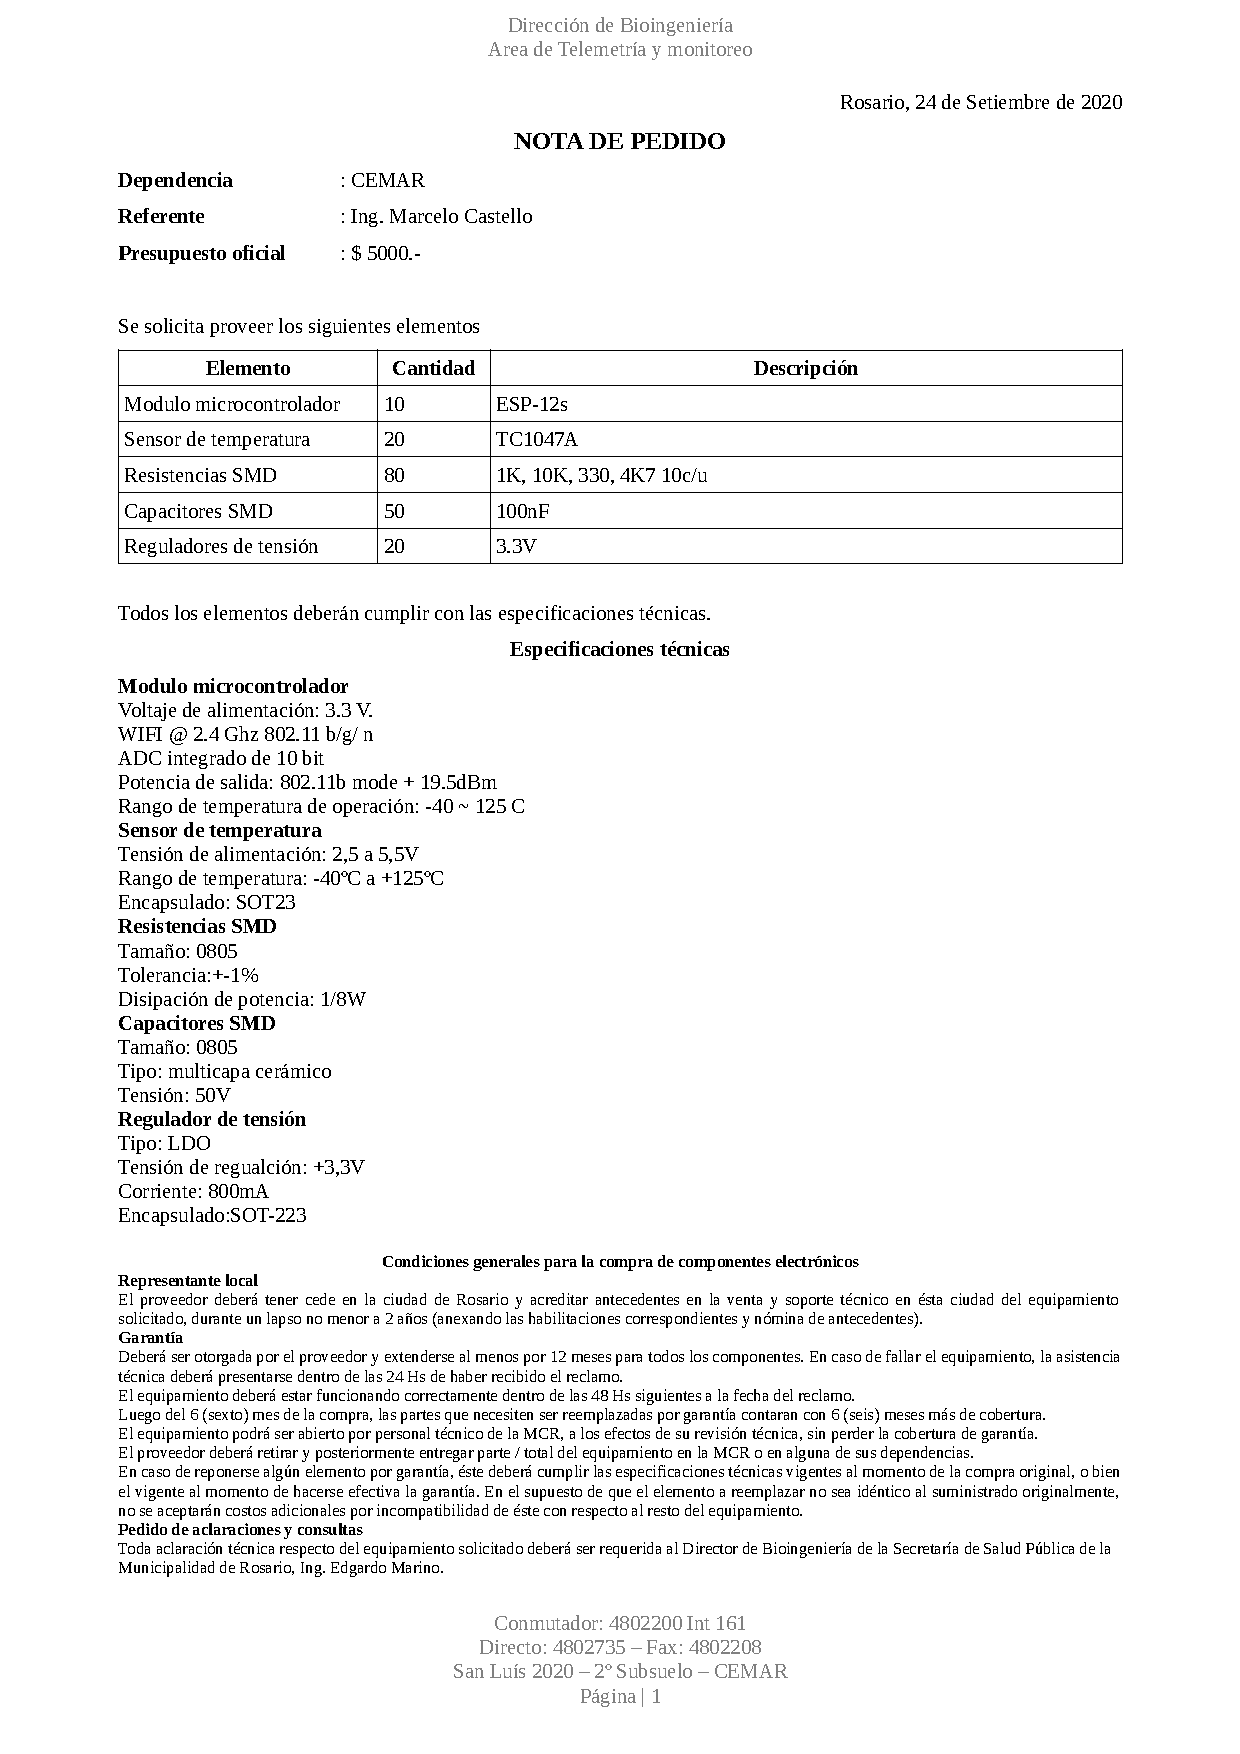
\includegraphics[width=1\textwidth]{./Figuras/nota_pedido.pdf}
\caption{\textit{Nota de pedido para compra directa}}
\label{nota_pedido}
\end{figure}


\begin{figure}[htpb]
\centering 
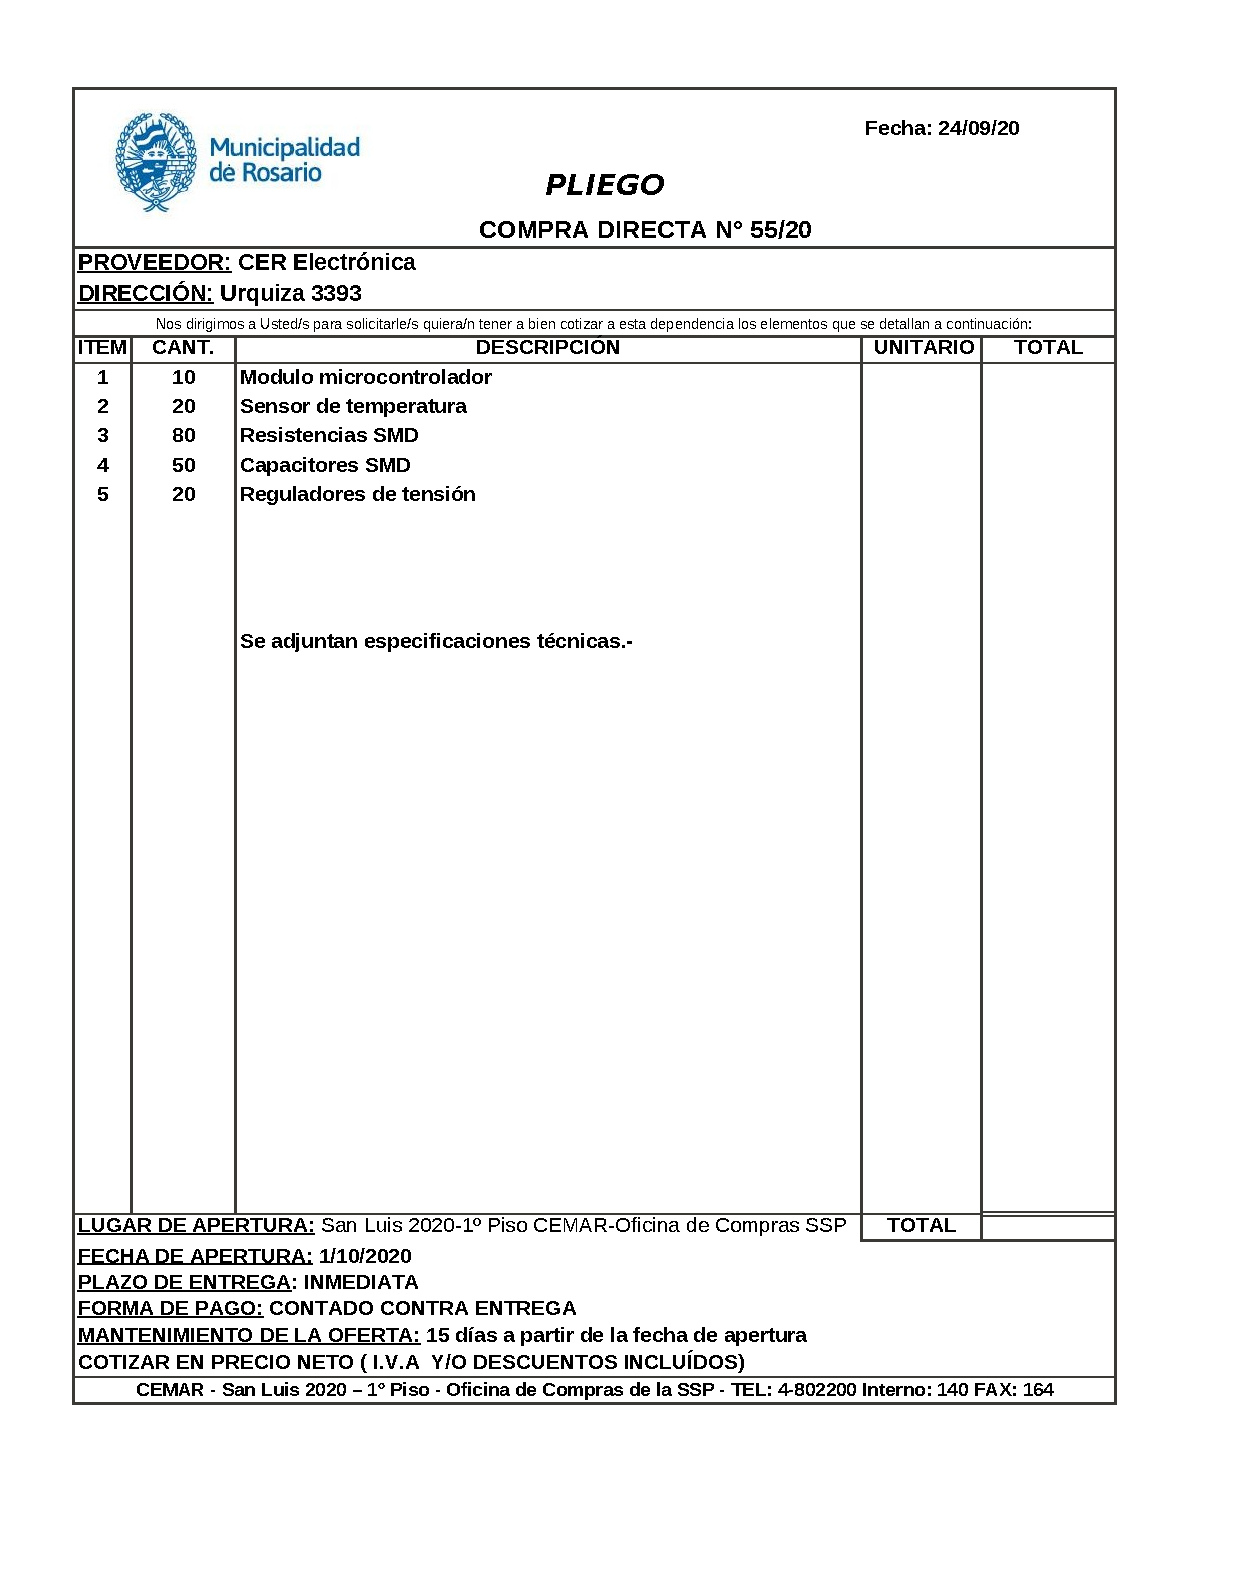
\includegraphics[width=1\textwidth]{./Figuras/compra_directa.pdf}
\caption{\textit{Pliego para compra directa}}
\label{compra_directa}
\end{figure}

\section{16. Seguimiento y control}
\label{sec:seguimiento}


\begin{longtable}{|m{1cm}|m{3.5cm}|m{2.2cm}|m{2cm}|m{3cm}|m{1.5cm}|}
\hline
\rowcolor[HTML]{C0C0C0} 
\multicolumn{6}{|c|}{\cellcolor[HTML]{C0C0C0}SEGUIMIENTO DE AVANCE}                                                                       \\ \hline
\rowcolor[HTML]{C0C0C0} 
Tarea del WBS 			& Indicador de avance & Frecuencia de reporte & Resp. de seguimiento & Persona a ser informada & Método de comunic. \\ \hline
\endfirsthead

\hline
\rowcolor[HTML]{C0C0C0} 
\multicolumn{6}{c}{\cellcolor[HTML]{C0C0C0}SEGUIMIENTO DE AVANCE}                                                                       \\ \hline
\rowcolor[HTML]{C0C0C0} 
Tarea del WBS 			& Indicador de avance & Frecuencia de reporte & Resp. de seguimiento & Persona a ser informada & Método de comunic. \\ \hline
\endhead

\multicolumn{6}{c}{Continúa}
\endfoot

\endlastfoot

1.1 & Finalización &Única Vez  &\authorname  &\supname &Correo    \\ \hline
 1.2 &  Finalización & Única Vez &\authorname  &\supname, \clientename &  Correo\\ \hline
 1.3& Finalización & Única Vez &\authorname  &\supname, \clientename &  Correo\\ \hline
 1.4&Cada reunión & Diaria &\authorname  &\supname, \clientename &  Correo\\ \hline
 1.5& Elección de la aplicación& Única Vez &\authorname  &Roberto Collelo  &Reunión\\ \hline
 1.6&   Cada capítulo &Semanal  &\authorname  &\supname &Correo    \\ \hline
 2.1& Elección del sensor &Única Vez &\authorname  &Roberto Collelo &Reunión\\ \hline
 2.2& Cada simulación &Diaria&\authorname  &Roberto Collelo &Reunión\\ \hline
 2.3&Cada prueba &Diaria&\authorname  &Roberto Collelo &Reunión\\ \hline
 2.4&Elección del dispositivo &Única Vez &\authorname  &Roberto Collelo &Reunión\\ \hline
 2.5&Biblioteca elegida &Única Vez &\authorname  &Roberto Collelo &Reunión\\ \hline
 2.6&Avance del diseño &Semanal &\authorname  &Roberto Collelo &Reunión\\ \hline
 2.7& Cantidad de placas montadas   &Diaria&\authorname  &Roberto Collelo &Reunión\\ \hline
 3.1&Biblioteca elegida &Única Vez &\authorname  &Roberto Collelo &Reunión\\ \hline
 3.2& Cerificado generado &Única Vez &\authorname  &Roberto Collelo &Reunión\\ \hline
 3.3& Cada función probada & Semanal &\authorname  &Roberto Collelo &Reunión\\ \hline
 3.4& Finalización & Única Vez &\authorname  &\supname, Roberto Collelo &Reunión\\ \hline
 3.5& Finalización & Única Vez &\authorname  &Roberto Collelo &Reunión\\ \hline
 3.6& Cada página & Semanal &\authorname  &Roberto Collelo &Reunión\\ \hline
 3.7& Finalización & Única Vez &\authorname  &\supname, Roberto Collelo &Reunión\\ \hline
 3.8& Cada incidencia & Semanal &\authorname  &Roberto Collelo &Reunión\\ \hline
 4.1& Finalización & Única Vez &\authorname  &\supname &Correo\\ \hline
 4.2& Finalización & Única Vez &\authorname  &\supname &Correo\\ \hline
 5.1& Finalización & Única Vez &\authorname  &\supname &Correo\\ \hline
 5.2& Finalización & Única Vez &\authorname  &\supname &Correo\\ \hline
 5.3& Finalización & Única Vez &\authorname  &\supname &Correo\\ \hline
 5.4& Cada panel &Semanal &\authorname  &\supname, Roberto Collelo &Reunión\\ \hline
 5.5& Cada prueba & Semanal &\authorname  &\supname, \clientename &  Correo\\ \hline
 6.1& Cada canal creado &Semanal &\authorname  &Roberto Collelo &Reunión\\ \hline
 6.2& Finalización & Única Vez &\authorname  &\supname, \clientename &  Correo\\ \hline
 6.3& Cada regla &Semanal &\authorname  &Roberto Collelo &Reunión\\ \hline
 6.4&  Cada regla &Semanal &\authorname  &Roberto Collelo &Reunión\\ \hline
 6.5& Cada alarma  &Semanal &\authorname  &Roberto Collelo &Reunión\\ \hline
 6.6& Cada alarma &Semanal &\authorname  &Roberto Collelo &Reunión\\ \hline
 7.1& Finalización & Única Vez &\authorname  &\supname, \clientename &  Reunión\\ \hline
 8.1& Cada capítulo &Semanal&\authorname  &\supname &  Correo\\ \hline
 8.2& Cada capítulo &Semanal&\authorname  &\supname &  Correo\\ \hline
 8.3& Cada slide &diaria&\authorname  &\supname &  Correo\\ \hline




\end{longtable}


\section{17. Procesos de cierre}    
\label{sec:cierre}

Las actividades de los procesos de cierre estarán a cargo del responsable del proyecto, \authorname .

\begin{itemize}
\item Se analizará el grado de cumplimiento del plan de trabajo en contraste con su ejecución. Se detectarán aquellas tareas que no se cumplieron en tiempo y se hará su correspondiente evaluación a fin de tener esta información en cuenta para otros proyectos. Esta documentación será guardada en el repositorio Git del proyecto.

\item Se compararán los resultados obtenidos con los requerimientos planteados en el plan original. De haber diferencias se analizarán, para observar si los mismos estuvieron correctamente planteados.


\item Se identificarán las técnicas que han sido especialmente útiles de la planificación y aquellas que no fueron de utilidad y se documentará en el repositorio de Git esta valiosa información para su uso en futuros proyectos.

De la misma manera, se documentarán en repositorio los problemas surgidos y sus soluciones.

\item Una vez presentado el trabajo ante el jurado, se realizará un agradecimiento público al
director y a todas las personas que hayan estado involucradas en el proyecto.

\end{itemize}






\end{document}
